%%%%%%%% ICML 2025 EXAMPLE LATEX SUBMISSION FILE %%%%%%%%%%%%%%%%%

\documentclass{article}
% Recommended, but optional, packages for figures and better typesetting:
\usepackage{microtype}

% Comment out the following line for the final version to render images 
\usepackage{graphicx}
%\usepackage[draft]{graphicx}

\usepackage{booktabs} % for professional tables
\usepackage{placeins} % Add this to your preamble
\usepackage{tabularx}  % For full-width tables
\usepackage{svg}

% hyperref makes hyperlinks in the resulting PDF.
% If your build breaks (sometimes temporarily if a hyperlink spans a page)
% please comment out the following usepackage line and replace
% \usepackage{icml2025} with \usepackage[nohyperref]{icml2025} above.
\usepackage{hyperref}


% Attempt to make hyperref and algorithmic work together better:
\newcommand{\theHalgorithm}{\arabic{algorithm}}

% Use the following line for the initial blind version submitted for review:
\usepackage{icml2025}

% If accepted, instead use the following line for the camera-ready submission:
% \usepackage[accepted]{icml2025}

% For theorems and such
\usepackage{amsmath}
\usepackage{amssymb}
\usepackage{mathtools}
\usepackage{amsthm}
\usepackage{subcaption}

% if you use cleveref..
\usepackage[capitalize,noabbrev]{cleveref}

%%%%%%%%%%%%%%%%%%%%%%%%%%%%%%%%
% THEOREMS
%%%%%%%%%%%%%%%%%%%%%%%%%%%%%%%%
\theoremstyle{plain}
\newtheorem{theorem}{Theorem}[section]
\newtheorem{proposition}[theorem]{Proposition}
\newtheorem{lemma}[theorem]{Lemma}
\newtheorem{corollary}[theorem]{Corollary}
\theoremstyle{definition}
\newtheorem{definition}[theorem]{Definition}
\newtheorem{assumption}[theorem]{Assumption}
\theoremstyle{remark}
\newtheorem{remark}[theorem]{Remark}

% Todonotes is useful during development; simply uncomment the next line
%    and comment out the line below the next line to turn off comments
%\usepackage[disable,textsize=tiny]{todonotes}
\usepackage[textsize=tiny]{todonotes}


% The \icmltitle you define below is probably too long as a header.
% Therefore, a short form for the running title is supplied here:
\icmltitlerunning{Local Loss Landscape Decomposition}

\begin{document}

\twocolumn[
\icmltitle{Identifying Sparsely Active Circuits Through Local Loss Landscape Decomposition}

% It is OKAY to include author information, even for blind
% submissions: the style file will automatically remove it for you
% unless you've provided the [accepted] option to the icml2025
% package.

% List of affiliations: The first argument should be a (short)
% identifier you will use later to specify author affiliations
% Academic affiliations should list Department, University, City, Region, Country
% Industry affiliations should list Company, City, Region, Country

% You can specify symbols, otherwise they are numbered in order.
% Ideally, you should not use this facility. Affiliations will be numbered
% in order of appearance and this is the preferred way.
\icmlsetsymbol{equal}{*}

\begin{icmlauthorlist}
\icmlauthor{Brianna Chrisman}{equal,a}
\end{icmlauthorlist}

\icmlaffiliation{a}{Independent}
\icmlauthor{Brianna Chrisman}{equal,a}


\icmlcorrespondingauthor{Brianna Chrisman}{brianna.chrisman@gmail.com}


% You may provide any keywords that you
% find helpful for describing your paper; these are used to populate
% the "keywords" metadata in the PDF but will not be shown in the document
\icmlkeywords{Machine Learning, ICML}

\vskip 0.3in
]

% this must go after the closing bracket ] following \twocolumn[ ...

% This command actually creates the footnote in the first column
% listing the affiliations and the copyright notice.
% The command takes one argument, which is text to display at the start of the footnote.
% The \icmlEqualContribution command is standard text for equal contribution.
% Remove it (just {}) if you do not need this facility.

%\printAffiliationsAndNotice{}  % leave blank if no need to mention equal contribution
%\printAffiliationsAndNotice{\icmlEqualContribution} % otherwise use the standard text.

\begin{abstract}

\end{abstract}

\section{Background}


Mechanistic interpretability is somewhat of an emerging field and aims to uncover the internal mechanisms responsible for seemingly black box behavior of large models so that developers can better understand, intervene on, and align model \cite{bereska2024mechanistic}. Within mechanistic interptretabilty, decomposition methods aim decompose model behacvior into subcomponents that are less complex and more human interpretabile, but that still fully express model behavior. The most popular method in this space is Sparse Autoencoders, which have been successful in decomposing compressed features in the activation space of a model \cite{gao2024scaling,cunningham2023sparse,bricken2023towards}.

\subsection{Limitations of Activation Space-Based Methods}

Sparse autoencoders rely on the activation space of a model, the output of a set of model's neurons during inference. Sparse autoencoders (SAEs) are designed to identify latent features by projecting a model's compressed activation space into a sparsely activated, overcomplete basis. These learned basis vectors represent distinct features, which can then be used to reconstruct the original activations.

Despite their utility, activation-based decomposition methods like SAEs have notable limitations. First, they assume that activation space consists of linear combinations of feature vectors, yet growing evidence suggests that even architectures designed to encourage linearity, such as residual streams, may encode non-linear features \cite{engels2024not,engels2024decomposing}. Second, activation-based approaches generally treat layers and blocks as independent computational modules, reconstructing activations from specific layers without capturing the possibility of cross-layer interactions and superposition \cite{merullo2024talking,lindsey2024sparse}. This limitation is particularly problematic in architectures beyond transformers, such as recurrent networks, adversarial networks, diffusion models, and classic RL models, where the separation of activation spaces is even less well-defined \cite{pascanu2013difficulty,goodfellow2014generative,ho2020denoising,mnih2015human}. Finally, activation-based methods provide little insight into how features emerge during training, making it difficult to link learned behaviors to specific data or optimization dynamics. This lack of connection to the training process limits our ability to intervene in model behavior at an early stage or refine training data to steer a model toward more desirable properties.


\subsection{Loss Landscape Geometry}

An alternative to interpreting models through their activations is to interpret models through their loss landscape geometry, understanding how perturbing parameters, rather than activations, affects model output and behavior. Parameters are the fundamental entities updated during training, capturing information from data in a way that persists beyond individual inferences. Unlike activations, which are transient and input-dependent, the parameter space reflects the cumulative outcome of the training process, potentially providing deeper insights into how models generalize, store knowledge, and develop internal representations.

A growing body of research explores the relationship between parameter space, data, and model behavior. Singular learning theory (SLT) describes how the structure of high-dimensional parameter space influences generalization and feature formation \cite{watanabe2007almost,watanabe2000algebraic,watanabe2005algebraic,wei2022deep}, while developmental interpretability extends this by analyzing how parameter updates evolve over training\cite{sharkey2025open}. Studying parameter space has already led to key insights, such as the role of sharpness in grokking\cite{davies2023unifying}, phase transitions corresponding to important learning stages in language models\cite{wang2024loss,hoogland2024developmental}, and distinctions between parameters associated with memorization vs. generalization\cite{bushnaq2024using}. These findings suggest that parameter-space analysis may uncover mechanisms that activation-based methods overlook, opening new avenues for interpretability and intervention.

\subsection{Degenerate Loss Landscapes}

We already know that loss landscapes have high levels of degeneracy. Mathematical degeneracy, data distribution degeneracy, etc. We hypothesize that 

\subsection{Contrastive Methods}
Constrastive/paired methods are common in intepretability. They work


\subsection{Loss Landscape Decomposition}


We propose a method for identifying features and the circuits that produce them in large models by analyzing parameter space rather than activations. Our approach identifies directions in parameter space that correspond to specific circuits, drawing on insights from singular learning theory (SLT). Our method aims to identify principle directions in parameter space such that for a given sample, moving model parameters in most of these directions will not meaningfully change the model's output, but for a small subset of directions, the model's output will change dramatically. We hypotheize that these directions, or subnetworks, represent distinct computations. 

To our knowledge, there have only been two prior methods attempting to decompose parameter space for interpretability. In one earlier work\cite{matena2023npeff}, the authors decompose parameter space by computing principal directions of a per-sample Fisher Information matrix to resolve meaningful features. This approach aimed to identify parameter directions most sensitive to individual samples, capturing how different parts of the model contribute to specific tasks. However, due to computational constraints, it relied on diagonalization techniques to approximate key directions, which limited its ability to fully capture sparse, structured circuits. Another recent method, \cite{braun2025interpretability} to is Attribution Parameter Decomposition (APD), which uses a bi-optimization approach to identify subnetworks where (1) the sum of subnetwork weights is close to the original model parameters, and (2) for any given input, the sum of a smaller set of subnetworks - identified through topk attribution values - has low behavioral loss when compared to the original model.  

%--------------------- FIGURE 1: Jacobian Diagram ---------------------
% Make two figures on top of each other
% use svgs

\begin{figure}
    \begin{subfigure}{\columnwidth}
        \centering
        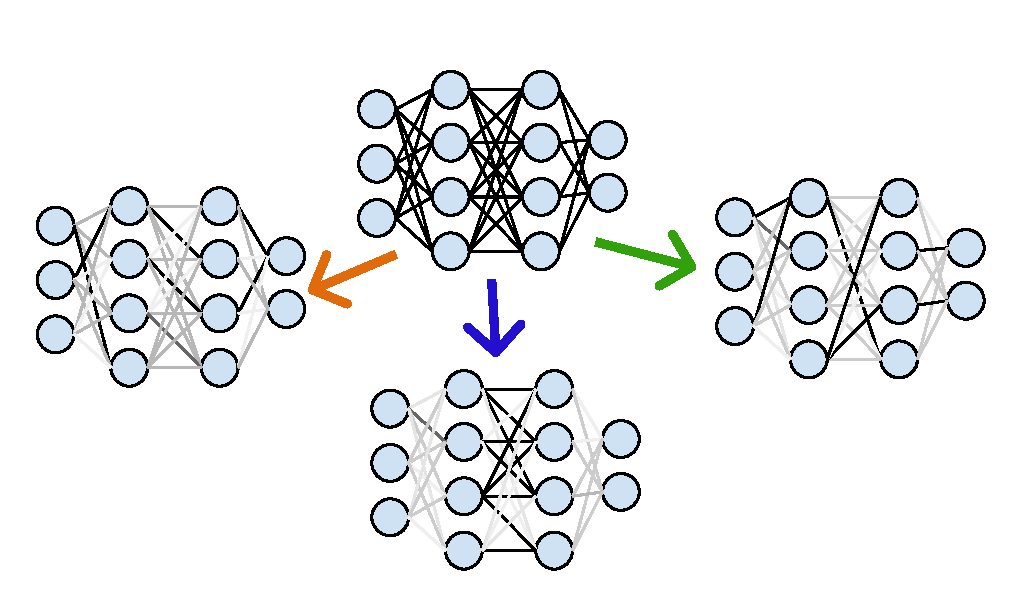
\includegraphics[width=.7\textwidth]{../figures/1b_jacobian_diagram.pdf}
    \end{subfigure}
    \begin{subfigure}{\columnwidth}
        \centering
        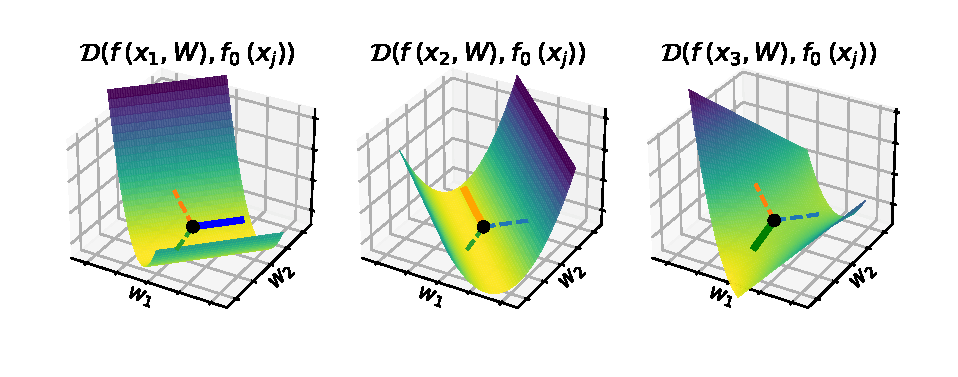
\includegraphics[width=\textwidth]{../figures/1a_jacobian_diagram.pdf}
    \end{subfigure} \caption{Decomposing a loss landscape into a set of principal directions , where (1) the set of directions can approximately reconstruct any per-sample Jacobian and (2) for any given sample, the curvature in most of the principle directions is approximately zero.}\label{fig:1_jacobian_diagram}
    
\end{figure}


Local loss landscape decomposition (L3D) aims to decompose a model's gradients of loss between output pairs with respect to parameter space \ref{fig:1_jacobian_diagram}. We seek to identify directions in parameter space such that (1) the set of directions can approximately reconstruct any gradient of paired sample divergences, and (2) for any given pair of samples, an even smaller subset of directions can be used in reconstructing this gradient. To reduce computational complexity, we learn low-rank representations of these parameter directions. In this work, we first describe the mathematical foundation of our approach. We then develop progressively more complex toy models to measure the efficacy of L3D and quantify its limitations. %Finally, we apply L3D to a real-world model to derive insights into model computation that would not have been possible through activation-based methods. We discuss the strenghts and limitations of L3D, and what we see as future work. 


\section{Methodology}


\subsection{Set up}

Our project rests on the following premise: For a given input, there are many components of a model that are not involved in inference. Changing these parameters will not affect change the model's output. For the same given input, there are a smaller set of components in a model that are highly involved in inference. Changing these parameters will change the model's output, and will do so in a meaningful way - it will effectively turn a circuit "up" or "down", pushing the model's output towards the value that would be output if the model had never learned that specific circuit. 

To formalize this, we will consider a model $f(x, W) ~ R^{n_s \times n_f} \mapsto R^{n_s \times n_o}$ that takes an input $x$ and parameter values of $W$ and outputs a vector of outputs values.

We wish to find a set of directions $V$ in parameter space, such that for any given sample, a small set of these directions can be used to express the parameter directions that meaningfully change the model's output. 

In the next sections, we will define "meaningful" changes, describe how to efficiently decompose parameters into these directions, explain a training algorithm for learning such a decomposition, and then explain how to use these decompositions to intervene on a model's behavior. 

\subsection{Divergences of Paired Outputs}
We wish to identify parameter directions that can be thought of as modular circuits. We would like to identify circuits that we can intervene on, and control individual computations, without fully breaking a model. Put another way, intervening in a certain parameter direction should not move our outputs too far away from the original output distribution.  

The object we will be decomposing is the gradient of divergence between a pair of outputs. 

Divergence of a pair of outputs can be defined as:
\begin{align}
    &\nabla_w D(f(x_i, W), f(x_r, W_0))|_{W=W_0} \\
    &\text{ where } x_i, x_r \in X
\end{align}


Note that we will abbreviate $f(x_r, W_0)$ as just $f(x_r)$ from here on out.

where $D$ is a divergence measuer, $f$ is our model, $x_i$ is our input of interest, $x_r$ is a randomly selected reference input , $W$ is a set of parameters and $W_0$ is the model's parameters after training. For our toy models we use MSE divergence. $x_i$ and $x_r$ are fixed for a given pair.

 We are interested in identifying directions in parameter space that move the model's output within the same subspace that the original model's output lies. This is why we look at divergence with a reference output $x_r$. We will be interested in decomposing gradient of this divergence with respect to the parameters $W$. For short, we will call this $\nabla_W D$

\begin{equation}
    \nabla_W D = \nabla_W D(f(x_i, W), f(x_r))|_{W=W_0}
\end{equation}

\subsection{Sparse Principal Directions}
We want to transform our gradient into components that represent directions in parameter space, where each sample's gradient can be written as a linear combination of a small set of these components. Formalizing this:

We want to find transforms $V^{in} ~ R^{n_v \times n_w}$ and $V^{out} ~ R^{n_w \times n_v}$ where $n_w$ is the number of parameters in the model, and $n_v$ is the number of components we wish to use to represent the parameter space.

\begin{align}
    & \nabla_W D \approx {V^{out}}_{:, topK} {V^{in}}_{topK,:} \nabla_W D \\
    & \text{ where } topK = \text{argtopK} abs({V^{in}} \nabla_W D)
\end{align}


$topK$ is a hyperparameter that controls the number of components we wish to use to reconstruct each sample. In practice, we use a batchTopK \cite{} and a fraction rather than an absolute number.


\subsubsection{Low Rank parameter directions}
Learning full rank parameter circuits would be extremely expensive, and we expect that modular, sparsely active circuits would be lower rank that their full-model counterparts \cite{}. Therefore, we use low-rank representations of our $V^{in}$ and $V^{out}$, and correspondingly learn low-rank circuits. 

While $W$ is a vector of all of the parameters in a model, typically model parameters are organized into tensors $W=\{w_i\}_i$. 

If our parameters are organized into tensors $W=\{w_i\}_i$, each subnetwork or parameter component can be organized as $V^{in}_i  = {\{{v^{in}}_i\}}_i, V^{out}_i = {\{{v^{out}}_i\}}_i$ where we have parts of our subnetworks corresponding to each tensor in the original model parameters. We wish each of these tensors to be low rank, and we express them using the canonical polyadic decomposition \cite{} (a way to write 3+ dimentinoal tensors in terms of low-rank components).

\begin{equation}
{v^{in}}_{i,j} = \sum_{r=1}^{R} a_{i,j,r} \times b_{i,j,r} \times c_{i,j,r} ...
\end{equation}

Where R is the rank we wish to use to represent the parameter component, and the number of factors (a, b, c,...) in the factorization is equal to the number of dimensions in the tensor $w_i$.


\subsection{Training}
We wish to learn the decomposition-related transforms $V^{in}$ and $V^{out}$ that minimize the topK reconstruction loss the gradient of divergence of pairs: 

\begin{equation}
    L = {|| \nabla_W D - {V^{out}}_{:, topK} {V^{in}}_{topK,:} \nabla_W D ||}_2^2
\end{equation}

% Algorithm 1
\begin{algorithm}
\caption{Training Algorithm}
\begin{algorithmic}[1]
\FOR{each epoch}
    \FOR{each $X$}
        \FOR {each $x_i$}
            \STATE Randomly select $x_r ~ X$
            \STATE $\nabla_w D[i] = \nabla_w D(f(x_i, W), f(x_r))|_{W=W_0}$
        \ENDFOR
        \STATE $\nabla_v D = {V^{in}}_{topK,:} \nabla_w D$
        \STATE thresh = topK(abs($\nabla_v D$))
        \STATE $\hat{\nabla}_w D = {V^{out}} (\nabla_v D \times (abs(\nabla_v D) > thresh))$
        \STATE $L = {|| \nabla_w D - \hat{\nabla}_w D ||}_2^2$
        \STATE $L.\text{backward()}$
    \ENDFOR
\ENDFOR
\end{algorithmic}
\end{algorithm}

\subsection{Measuring and Intervening}

Our learned subnetworks will just be the rows of $V^{out}$, reorganized into the same tensor structure as $W$.

If we wish to intervene using a single subnetwork, we can do so by updating the parameters in the direction of the subnetwork, multiplied by a scalar $\delta$. We can tune our model in the direction of subnetwork $v_i$, and compute predictions by evaluating:

\begin{equation}
    f(x, W + \delta v_i)
\end{equation}


We can quantify the impact of a subnetwork in two ways. First, we can compute the impact of a subnetwork on a pair of samples $x_i, x_j$, identyfing the subnetwork that, if intervened upon, would most strongly impact the the divergence of $x_i$'s outputs when compared to $x_j$. The impact of subnetwork $v_i$ on such a pair of samples, $I(v_i, x_i, x_j)$ can be measured by:

\begin{equation}
    I(v_i, x_i, x_j) = \\
    abs({V^{in}}_{i,:} \nabla_w D(f(x_i, W), f(x_j))|_{W=W_0})
\end{equation}

Secondly, we can average the impacts of a subnetwork $v_i$ and an input $x_i$ over many different reference samples to quantify the impact of the subnetwork on a single sample's predictions.

\begin{equation}
    I(v_i, x_i) = \frac{1}{n} \sum_{j=1}^{n} I(v_i, x_i, x_j)
\end{equation}


\section{Results}

We designed several toy models to test the efficacy of L3D.

\begin{table*}[htb]
    \centering
    \begin{tabularx}{\textwidth}{X X X X X}  % Adjusted for new column structure
        \toprule
         & Toy model of superposition & Circuit Superposition & Higher Rank Circuit Superposition & Complex Loss Landscape \\  
        \midrule

        \hline
        & 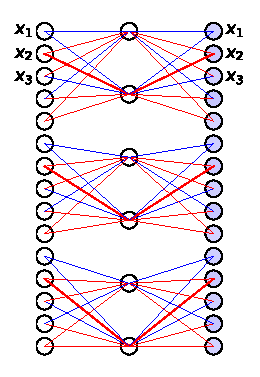
\includegraphics[width=0.12\textwidth]{../figures/2a_toy_models_setup.pdf} &
        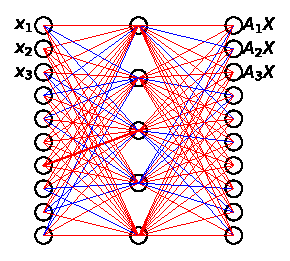
\includegraphics[width=0.2\textwidth]{../figures/2b_toy_models_setup.pdf} &
        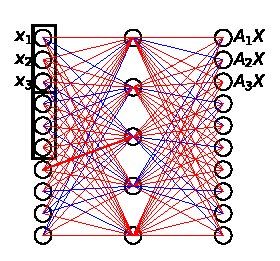
\includegraphics[width=0.2\textwidth]{../figures/2c_toy_models_setup.pdf} &
        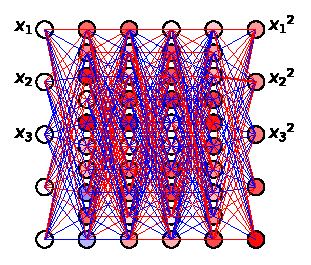
\includegraphics[width=0.2\textwidth]{../figures/2d_toy_models_setup.pdf} \\
         & $X \mapsto X$ & $X \mapsto A X$ & $X \mapsto A X$ & $X \mapsto X^2$ \\  
        Feature Superposition & $\checkmark$ & $\checkmark$ & $\checkmark$ & $\checkmark$ \\  
        Circuit Superposition & $\times$ & $\checkmark$ & $\checkmark$ & $\checkmark$ \\  
        Circuits $>$ rank-2 & $\times$ & $\times$ & $\checkmark$ & probably $\checkmark$ \\  
        Complex Loss Landscape & $\times$ & $\times$ & $\times$ & $\checkmark$ \\  
        \bottomrule
    \end{tabularx}
    \caption{Toy models and their properties (transposed)}
    \label{tab:toy_models_transposed}
\end{table*}

\subsection{Toy Model of Superposition}


\subsubsection{Setup}


We start off by validating our algorithm on a well-studied toy problem, the toy model of superposition (TMS), with a small variation. TMS is a single-layer autoencoder, where the number of input and output neurons are equal, and there is a smaller hidden layer in between, with a final relu activation function \cite{elhage2022toy}. The model is trained on a dataset of samples where few features are active at a time, and has been shown to "superimpose" these features in the hidden layer such that features embeddings in the hidden layer have minimal interference with each other. We train a toy model of superpsition with 5 features and 2 hidden dimensions (with 1-sparsity=.05), and then place three such models in parallel, to test our method's ability to resolve superimposed features, as well as indpendent circuit modules.



\subsubsection{Decomposition}
We use L3D to decompose the TMS model into 15 principal vectors, using rank-1   parameter tensors. We use topFrac=.1 and train L3D for 1000 epochs on 1000 datapoints. The network decomposes into subnetworks as we would expect: each subnetworks represents the embedding and reconstruction of a input $\mapsto$ output node, involving only the weights connecting the two and the biases of the output nodes. Figure \ref{fig:3_tms_subnetworks_first5} shows the subnetworks corresponding to each of the first 5 features, and Figure \ref{fig:s3_tms_full_subnetworks} shows the full decomposition.  One thing to note is that principal parameter vectors do not have a preferred direction. L3D is equally likely to identify a parameter vector in the direction of $\theta$ as it is in the direction of $-\theta$. This is why, for example, subnetwork 1 in Figure \ref{fig:3_tms_subnetworks_first5} has weights that are in the opposite direction as those in the original network.


This decomposition resulted in a reconstrcution error of \todo{Pull number form WandB}. 15 components of rank-1 can successfully express each individual $X_i:\hat{X}_i$ circuit, but does not capture the interference between features when multiple features are active in the same sample. Note that we expect decompositions of higher dimensional networks to exhhibit less reconstruction error, as the amount of nearly orthogonal parameter vectors (non-interferring) that can be compressed into parameter space scales exponentially with dimension.

%--------------------- FIGURE 2: TMS Subnetworks - First 5 ---------------------
\begin{figure*}
    \centerline{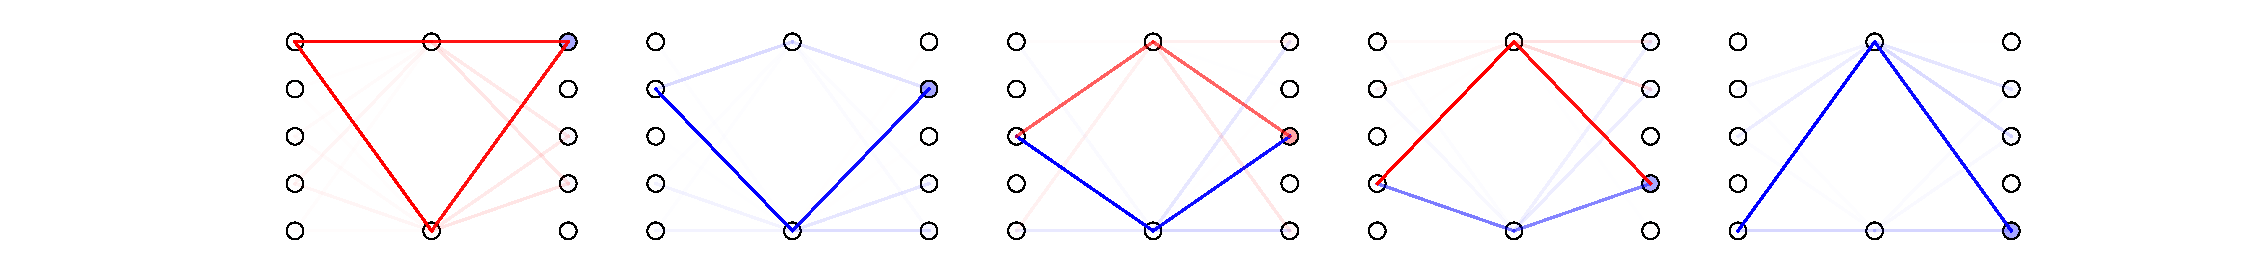
\includegraphics[width=\textwidth]{../figures/3_tms_first_5_subnetworks.pdf}}
    \centering
    \caption{Selected 5 subnetworks that L3D decomposes the TMS-in-parallel model into}\label{fig:3_tms_subnetworks_first5}
\end{figure*}


\subsubsection{Intervention}


Additionally, the low-rank parameter vectors learned by L3D can be used to perturb the weight space of a model. In principle, we could finetune a model with an adaptor that only changes the parameters of a network in the direction of a specified set of parameter vectors. Finetuning with a small set of parameter vectors should only affect the predictions of the samples for which those parameter vectors were active subnetworks. While we do not fine tune a model, we explore the effect of perturbing a model's weight space in the direction of a subnetwork. Moving the TMS-in-parallel model in the direction of a single subnetwork at a time has a limited effect on the predictinos of most samples, but does result in a significant change in the model's predictions for samples where we expect the subnetwork to be active. In fact, for TMS-in-parallel, we can successfully fully "turn off" a computation by moving far enough in the direction of the subnetwork (For model's with more complex loss landscapes, turning "off" a computation is not as straightforward, as we will later discuss).

%--------------------- FIGURE 4: TMS Intervention ---------------------
\begin{figure}
    \centerline{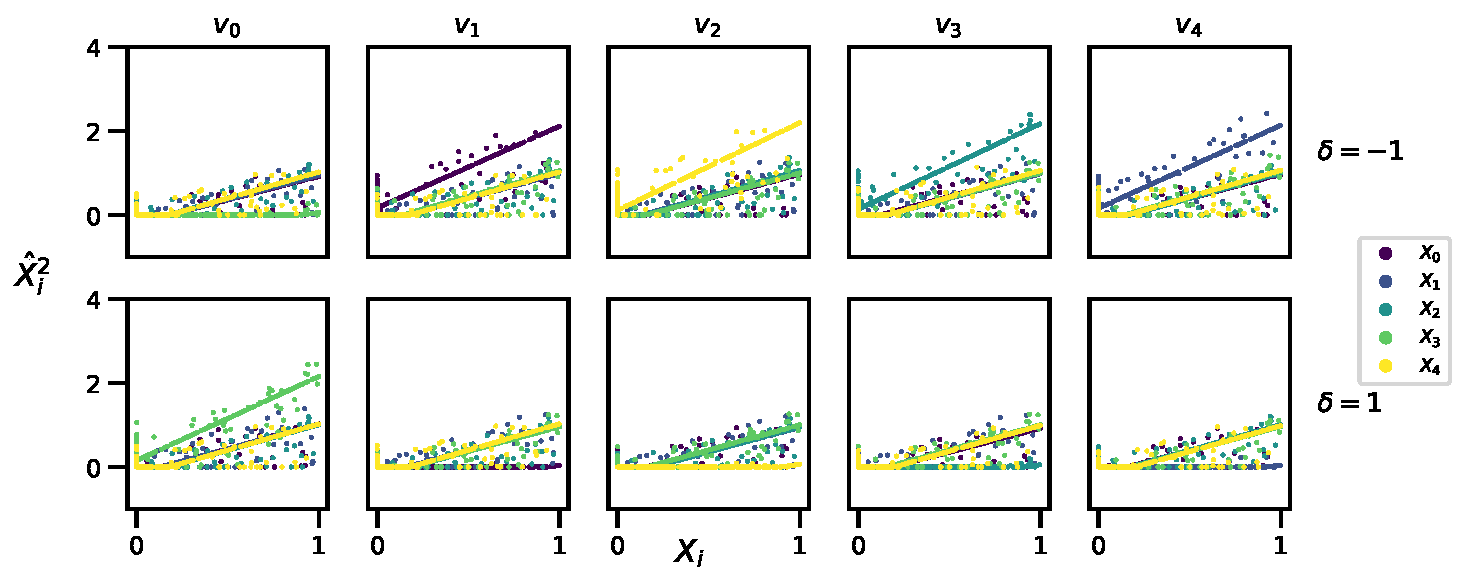
\includegraphics[width=\columnwidth]{../figures/4_tms_intervention.pdf}}
    \centering
    \caption{The effect of intervening on the TMS-in-parallel model in the direction of $\text{Network}_1$.}\label{fig:4_tms_intervention}
\end{figure}


\subsection{Toy Model of Circuit Superposition}

\subsubsection{Setup}


The toy model of superposition exhibits feature superposition - where features are represented by non-orthogonal activation vectors. However, the sparse circuits in TMS are noteably **not** in superposition - a given weight or parameter is only relevant for a single circuit. It seems highly unlikely that real world model circuits would decompose this way, since learning circuits composed of non-orthogonal parameter vectors would allow the model to put more expressivitiy into a compressed space. We therefore develop a toy model of **circuit superposition** (TMCS) in order to analyze L3D's ability to resolve such circuits. 

Our toy model of circuit superposition uses the same architeture and input data distribution as TMS, except our network is trained to predict linear combinations of the input features as its output, rather than reconstructions of each input feature ($X \mapsto A X$). We randomly select values of $A$ between 0 and 3 to generate input, output pairs to train the toy model with.

In this model, if we consider "subnetworks" to be parameter directions involved in inference of a small set of the input data, then we would expect each circuit to be associated with a single input feature. If this is the case, then parameters might be involved in multiple circuits: ${W^{dec}}_{i,1}$ (the set of parameters connecting the hidden nodes to the first output node) will contain information about both $A_{3,1}, A_{2,1}, A_{3,1}...$  Put another way, the circuits will interfere with each other - the parameter directions associated with each circuit will be non-orthogonal. 


\subsubsection{Decomposition}


Using rank-1 parameter tensor and 15 principal vectors, we decompose TMSC into 3 subnetworks (\ref{fig:5_circuit_superposition_decomposition}) (with \todo{PULL NUMBER FROM WandB} reconstruction error). Since each subnetwork theoretically corresponds to the computations involved with a single input feature, we should be able to reconstruct the original $A$ values from each subnetwork. To derive $A$ from each subnetwork, we (1) identify the which column in the subnetwork's $W^{dec}$ direction has the largest norm and then (2) trace the weights of the network through that path. That is for subnetwork $k$: 
\begin{align}
    &j^* = argmax_{j} ||{{{W^{dec}}_j}_k}||_2 \\
    &\hat{\alpha}_{i,j} = {{{W^{enc}}_{i,j}}}_k {{W^{dec}}_{i,j}}_k
\end{align}




%--------------------- FIGURE 5: Circuit Superposition ---------------------
\begin{figure*}[htbp]
    \centerline{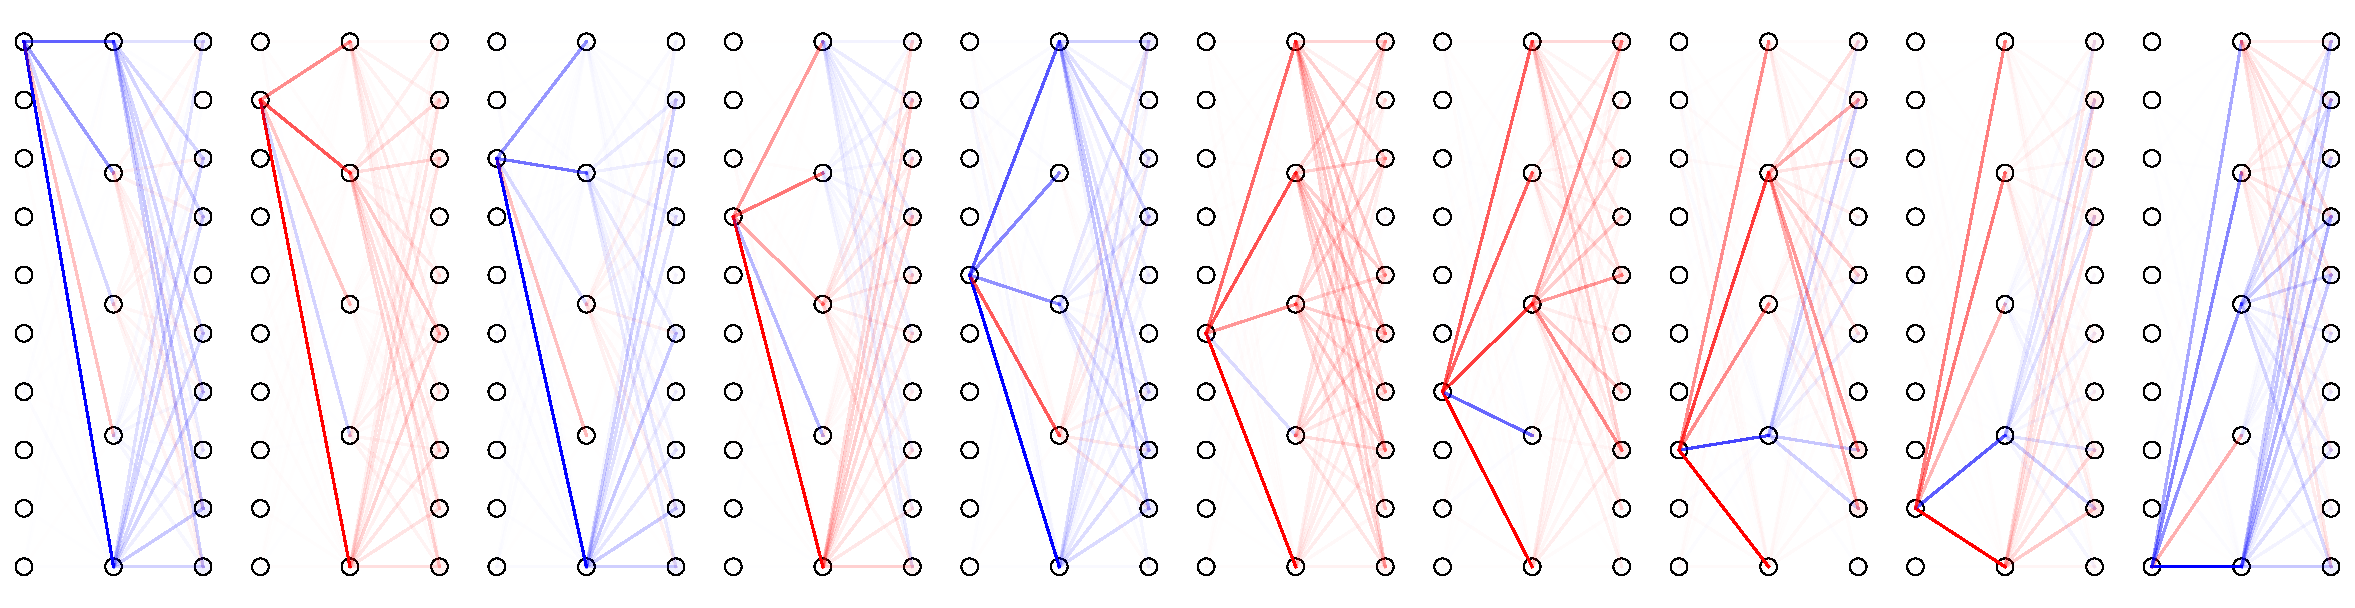
\includegraphics[width=\textwidth]{../figures/5_circuit_superposition_decomposition.pdf}}
    \centering
    \caption{The learned subnetworks of TMCS}\label{fig:5_circuit_superposition_decomposition}
\end{figure*}

The parameter vectors are normalized to be unit vectors so we expect them to be a scalar multiple of the true $\alpha$ values. As seen in Figure \ref{fig:5_circuit_superposition_decomposition}, our derived $\hat{\alpha}$ have a very high correlation to the original $\alpha$ values ($r^2 = 0.9$).

%--------------------- FIGURE 6: Circuit Superposition Coefficients ---------------------
\begin{figure}[htbp]
    \centerline{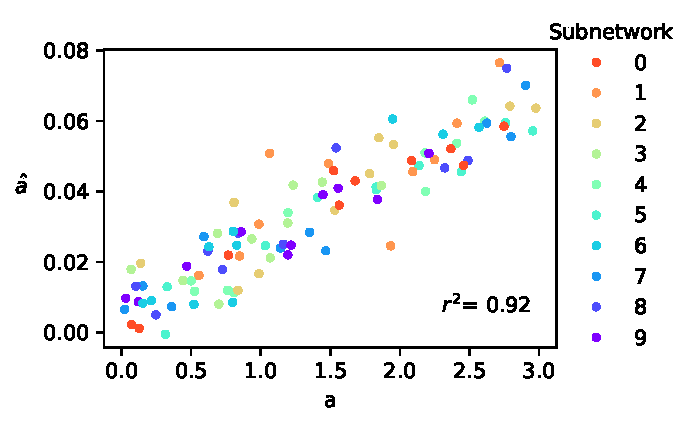
\includegraphics[width=\columnwidth]{../figures/6_circuit_superposition_coefficients.pdf}}
    \centering
    \caption{The coefficients derived from the subnetworks compared to actual coefficients}\label{fig:6_circuit_superposition_coefficients}
\end{figure}



\subsection{Higher Rank Circuits}

\subsubsection{Setup}
Because each subnetwork in TMSC traces the path of a single input neuron, the underlying subnetworks inherently have a rank of 1. In order to test the ability of L3D to learn higher rank circuits, and to understand the relationship between circuit rank and circuit superposition, we developed a toy model that inherently uses higher rank circuits (according to our definition of a circuit being sparsely involved in inference). For this model, we use the same set up as TMSC, but we correlate the sparsities of sets of input features. We use 24 input features, and we correlate the sparsities of the input features 1-5, 6-10, etc, ensuring that 1-3 are always active (>0) or inactive (<0) together. In this model, circuits should always be associated with groups of 5 input features and so should have a rank of 5.

TEST
\subsubsection{Decomposition}

Although we expect the model to have 6 subcircuits, we use excess parameter tensors (n=10) in order to allow more flexibility in learning. Futhermore, although we expect the underlying subcircuits to be rank-5, we experiment with using different rank representations to see how well lower-rank parameter directions can represent the model. Interestingly, rank-1 representations of the parameter tensors are able to represent the model nearly as well as rank-5 representations (Figure \ref{fig:s10_squared_decompositions_features}). Using a 10 rank-3 parameter representations, L3D successfully learns a subnetwork corresponding to each of the 6 sets of input features, as well as a number of "dead" or noisy subnetworks (Figure \ref{fig:s10_squared_decompositions_features}). The higher and lower rank decompositions learn similar subnetworks (Figure \ref{fig:s10_squared_decompositions_features}).



%--------------------- FIGURE 7: Higher Rank Circuit Superposition ---------------------
\begin{figure*}[htbp]
    \centerline{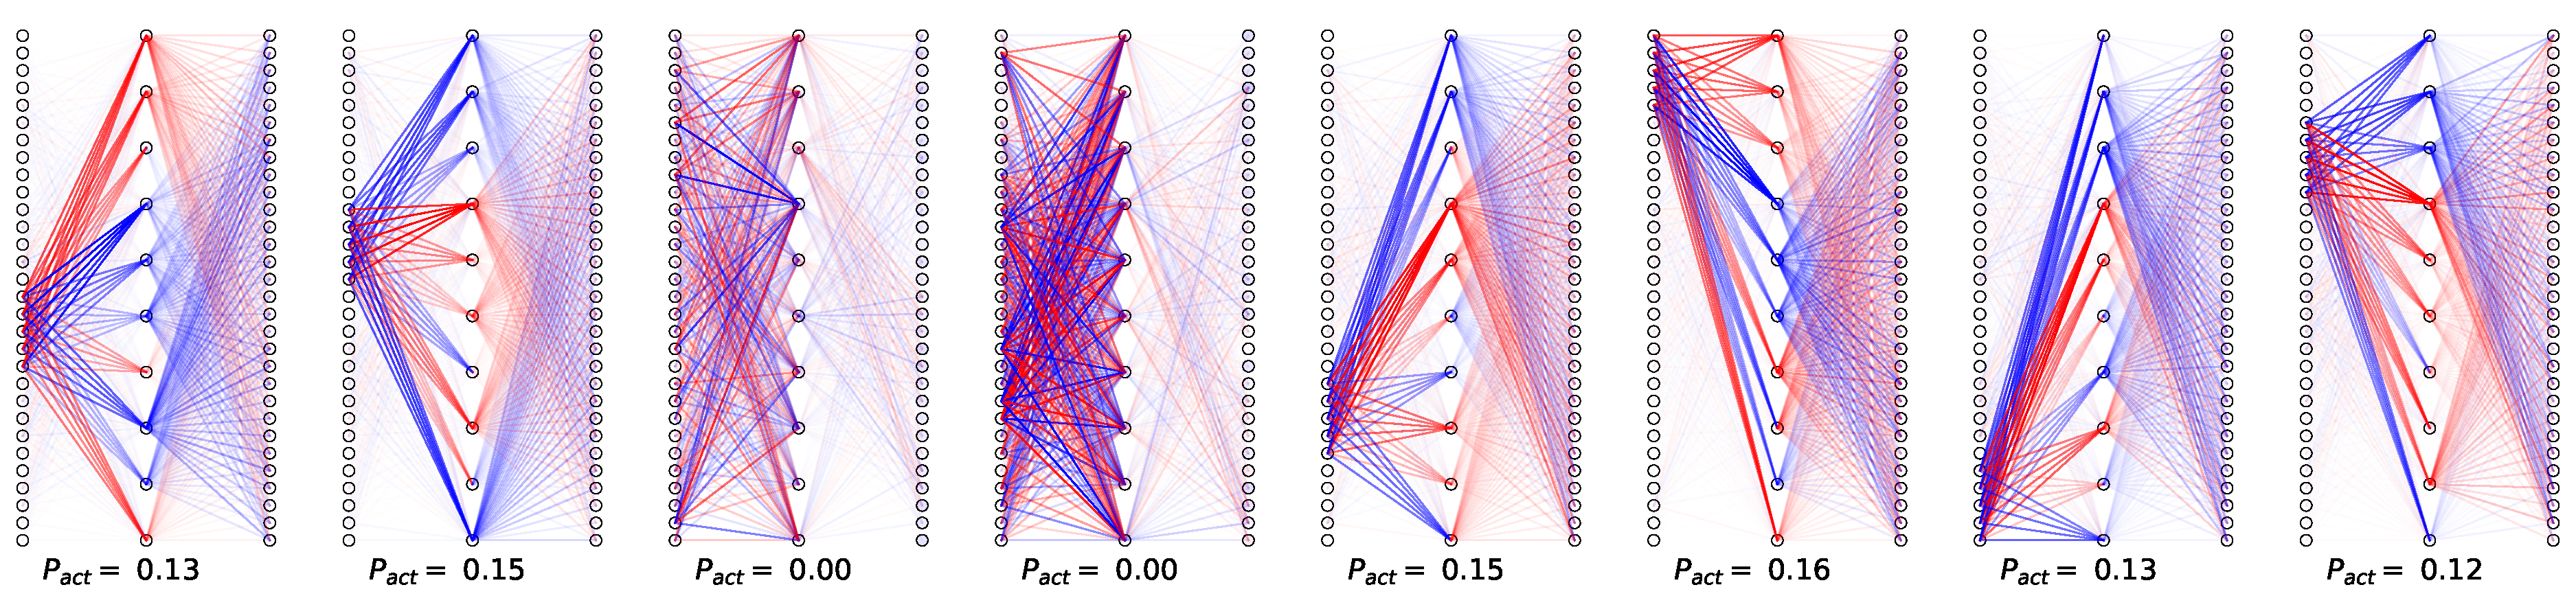
\includegraphics[width=\textwidth]{../figures/7_high_rank_decomposition.pdf}}
    \centering
    \caption{Parameter representations learned by L3D for the high rank circuit decomposition task.}\label{fig:7_high_rank_decomposition}
\end{figure*}


\subsection{Complex Loss Landscape}


\subsubsection{Setup}


The previous set of toy models all had quadratic landscapes with respect to $W^{enc}$ or $W^{dec}$ where $dMSE/dW_i$ depends on $W_i$ to the first order (or not at all, depending on whether the ReLU has fired)\todo{make sure this is right}. This suggests that the local loss landscape of the models will be a good approximation for much of the global loss landscape. However, we wanted to test the limitations of a L3D on a model with a more complex loss landscape, where we expect circuits to still be in superposition. 

We therefore trained a multi-layer model to predict multiple non-linear functions of input features at once. We train a GeLU network for $X_i \mapsto X_i^2$ . Specifically we use a network with 4 hidden layers of 5 neurons each, and 10 output and input input neurons. Once again, the input features are sparse, incentivizing the toy model to learn circuits in superposition whose interferences will cause minimal errors on the sparse input distribution. 

We expect the model to have 5 subnetworks, one for each input feature. While it is not entirely clear what rank the subnetworks should have, because this is a non-linear model we expect each tensor in the subnetwork to be full rank.

\subsubsection{Decomposition}

Given that rank-1 parameter tensors seemed to give reasonable representations of subcircuits in the previous model, we again use rank-1 parameter tensors for this model. Instead of varying rank, we experiment with using different numbers of subnetworks to represent our model. We decompose the model into sets of 3, 5, 10, and 15 subnetworks. In the 5-subnetwork decomposition (Figure \ref{fig:8_squared_subnetworks}), we see a subnetworks tracing the path of $X_i \mapsto X_i^2$ for each input feature $i$. In our 3-subnetwork decomposition, L3D still learned subnetworks corresponding to single input features, but can of course only represent 3 out of the 5 inputs. As we add more subnetworks, we are able to successfully learn more expressive decompositions of the model that lower reconstruction error (Figure \ref{fig:s10_squared_decompositions_features}). Interestingly, these subnetworks correspond to a combination of input and output-node specific subnetworks (ie network 0 in the 15-subnetwork decomposition), input-specific subnetworks (ie network 5), and output-specific subnetworks (ie network 8) \ref{fig:s10_squared_decompositions_features}.




\subsubsection{Intervention}

Intervening on these circuits helps us understand how much local loss landscape is representative of global loss landscape, particularly when it comes to inactive subnetworks remaining inactive as we move through parameter space. If local loss landscape is not representative of global loss landscape in this way, then intervening on a parameter direction of interest will result in a large number of samples being affected, rather than a small subset. \ref{fig:9_squared_intervention} shows our results for perturbing parameter directions. Even in this more complex toy model, local loss landscape is a relatively good approximation of the global loss landscape. We can perturb the parameters in a direction of interest and have a large impact on the predictions of that sample and a minor impact on others. If we perturb far enough, we do see some effects on the predictions of other samples, but ratio of change in predictions to the relevant samples to those of the irrelevant samples is very high.

A careful reader may have noticed is that it would be very easy to identify parameter directions in the first or last layer of the $X \mapsto X^2$ model involved in a sparsely active circuit. The circuit for $X_i \mapsto X_i^2$ would just involve all weights connecting input node $i$ to the first hidden layer, and all weights connecting the hidden node $i$ to the output node $i$, as well as the bias of output node $i$. In order to make sure L3D is not just learning this trivial solution, we want to make sure the hidden parameter directions it learns are also relevant for circuits. Therefore, from the learned parameter directions, we perform intervention experiments only interveining on the model's middle weights and biases. The results are very similar, where inventions on a parameter direction only affect the output of a subset of samples - showing that the circuits that L3D has learned perform relevant computation even in their middle layers. 

\ref{fig:9_squared_intervention} shows changes in predictions as we move in a single direction in parameter space. We'd also like to undrestand how subcircuits might interact with each other as we move through parameter space. In \ref{fig:s9_squared_intervention_multi_features} we perturb multiple subnetworks at once, and measure the new predictions. For the most part, the subnetworks have little inference with each other: the relevant output values for each subnetwork move relatively independently of each other. For some parameter directions, we do see some unexpected interactions, such as when we move in the direction of subnetwork 1 and 2, we see a small effect on the predictions of a few samples not associated with either subnetwork. With larger models, especially those with more modular circuits that are working together, we expect this kind of interaction to become more common. We discuss more in the discussion section. 

%--------------------- FIGURE 8: Squared Model Subnetworks ---------------------
\begin{figure*}[htbp]
    \centerline{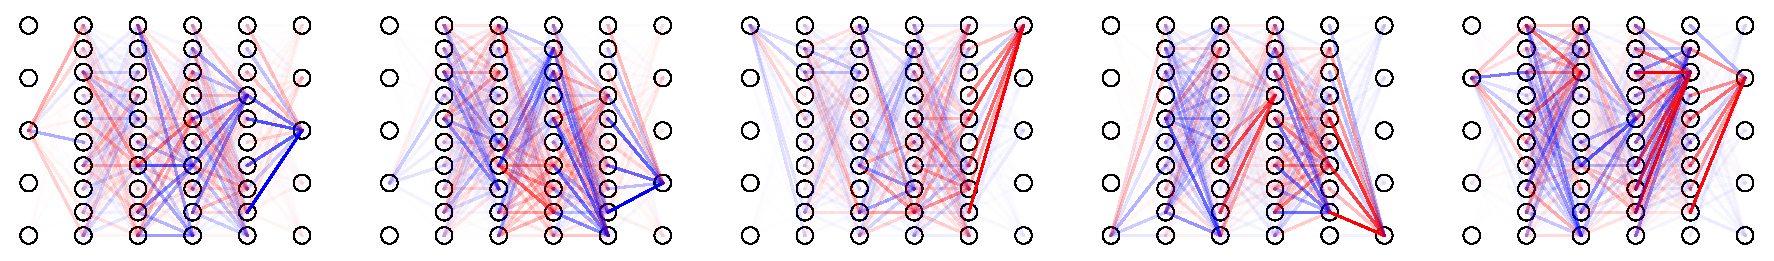
\includegraphics[width=\textwidth]{../figures/8_squared_subnetworks.pdf}}
    \centering
    \caption{Subnetworks learned by L3D for the $X \mapsto X^2$ model, and effect of intervening on each subnetwork}\label{fig:8_squared_subnetworks}
\end{figure*}


%----------------- FIGURE 9: Squared Subnetworks Intervention ------------------
\begin{figure*}[htbp]
    \centerline{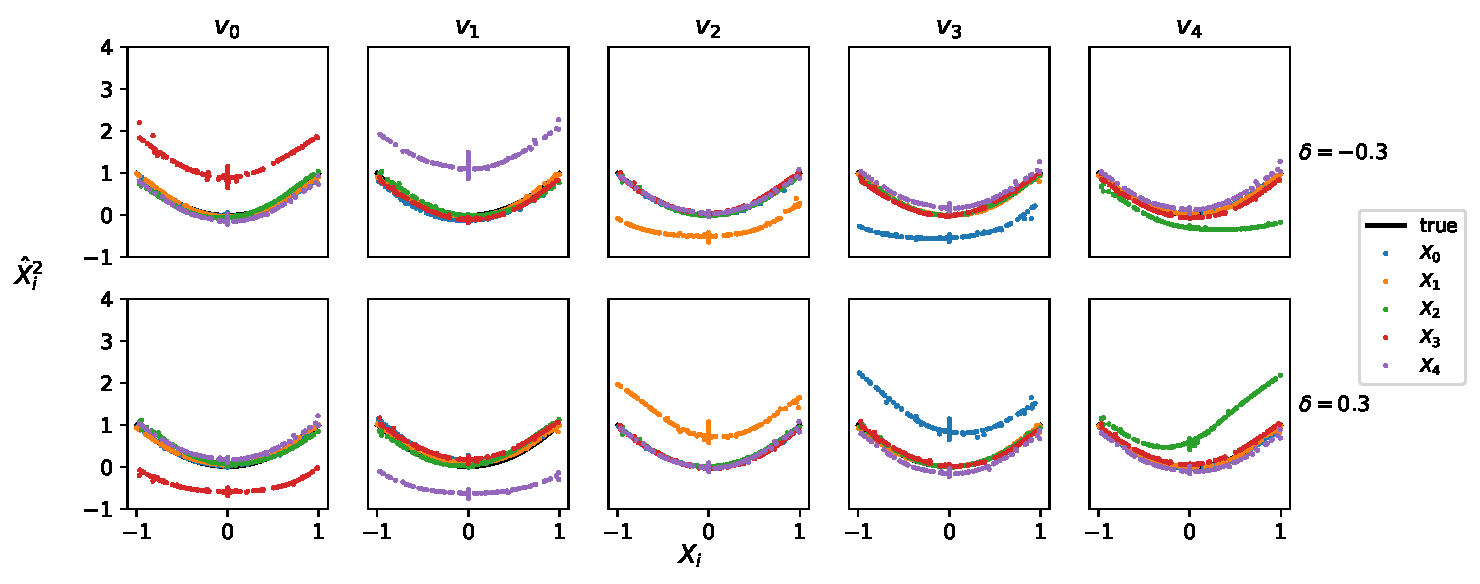
\includegraphics[width=\textwidth]{../figures/9_squared_intervention.pdf}}
    \centering
    \caption{The effect of intervening on each subnetwork}\label{fig:9_squared_intervention}
\end{figure*}


\section{Discussion}

Frankly crazy that local approximation works so well 

\subsection{Limitations}

\subsubsection{Hyperparameter Choice}

\subsubsection{Low Rank of blocks}

\subsubsection{Loss Landscape}
\subsection{Extensions}

\subsubsection{Finetuning}

\subsubsection{Identifying Specific Circuits with Constrastive Pairs}


 
\clearpage

\section*{Impact Statement}

%This paper presents work whose goal is to advance the field of 
%Machine Learning. There are many potential societal consequences 
%of our work, none which we feel must be specifically highlighted here.

% In the unusual situation where you want a paper to appear in the
% references without citing it in the main text, use \nocite

\clearpage
\bibliography{writeup.bib}
\bibliographystyle{icml2025}


%%%%%%%%%%%%%%%%%%%%%%%%%%%%%%%%%%%%%%%%%%%%%%%%%%%%%%%%%%%%%%%%%%%%%%%%%%%%%%%
%%%%%%%%%%%%%%%%%%%%%%%%%%%%%%%%%%%%%%%%%%%%%%%%%%%%%%%%%%%%%%%%%%%%%%%%%%%%%%%
% APPENDIX
%%%%%%%%%%%%%%%%%%%%%%%%%%%%%%%%%%%%%%%%%%%%%%%%%%%%%%%%%%%%%%%%%%%%%%%%%%%%%%%
%%%%%%%%%%%%%%%%%%%%%%%%%%%%%%%%%%%%%%%%%%%%%%%%%%%%%%%%%%%%%%%%%%%%%%%%%%%%%%%
\newpage
\appendix
\renewcommand{\thefigure}{S\arabic{figure}}  % Set figure numbers to S1, S2, etc.
\renewcommand{\theHfigure}{S\arabic{figure}} % Fix hyperlinks in hyperref
\setcounter{figure}{0}  % Reset numbering
\onecolumn


\section{Definitions}

\section{Additional Derivations}

\section{SupplementalFigures}


% ---------------------Figure S1 TMS subnetwork decomposition-------------------------
\begin{figure}[ht]
    \centerline{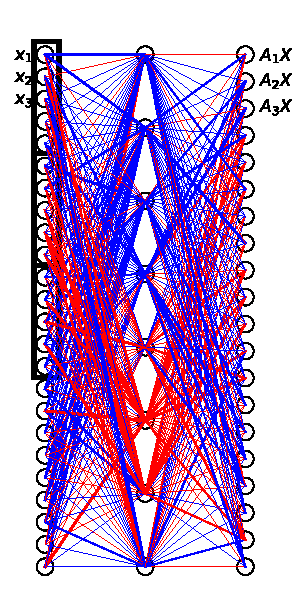
\includegraphics{../figures/s1_high_rank_circuit_setup.pdf}}
    \centering
    \caption{Full architecture of high rank circuit toy model.}\label{fig:s1_high_rank_circuit_setup}
\end{figure}



% ---------------------Figure S2 TMS subnetwork decomposition-------------------------
\begin{figure}[ht]
    \centerline{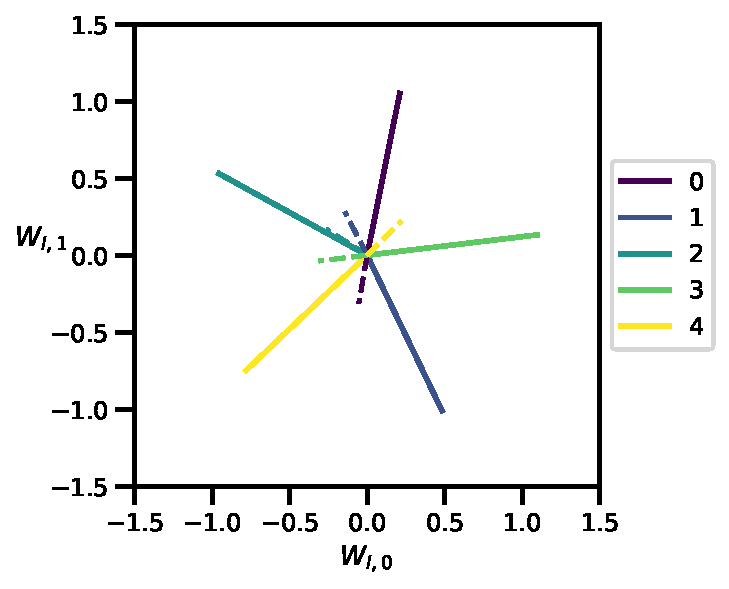
\includegraphics{../figures/s2_tms_encoder_directions.pdf}}
    \centering
    \caption{Encoder directions in TMS}\label{fig:s2_tms_encoder_directions}
\end{figure}


% ---------------------Figure S2 TMS subnetwork decomposition-------------------------
\begin{figure}[ht]
    \centerline{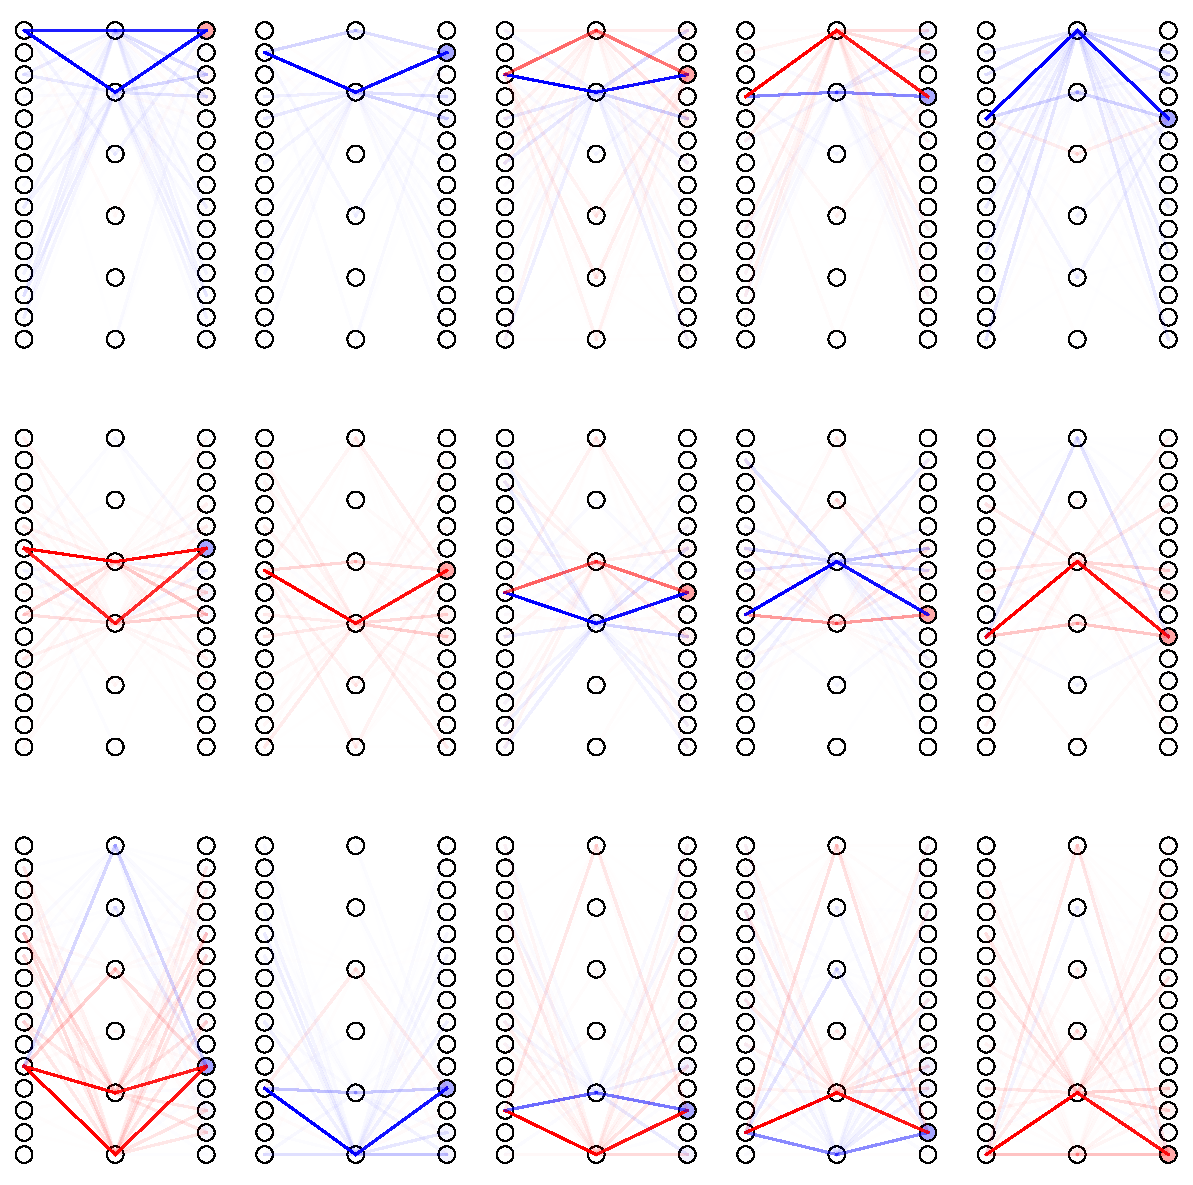
\includegraphics[width=\textwidth]{../figures/s3_tms_full_subnetworks.pdf}}
    \centering
    \caption{All subnetworks for the TMS decomposition}\label{fig:s3_tms_full_subnetworks}
\end{figure}


% ---------------------Figure S3: Intervention on TMS-in-parallel-------------------------
\begin{figure}[ht]
    \centering
    \caption{Effect of intervening on the first 5 subnetworks of the TMS-in-parallel model.}
    \label{fig:s3_tms_interventions}

    \begin{minipage}{\textwidth} % Ensure figures align
        \centering
        \begin{tabular}{cc}  % 3 columns
            \begin{subfigure}{0.3\textwidth}
                \centering
                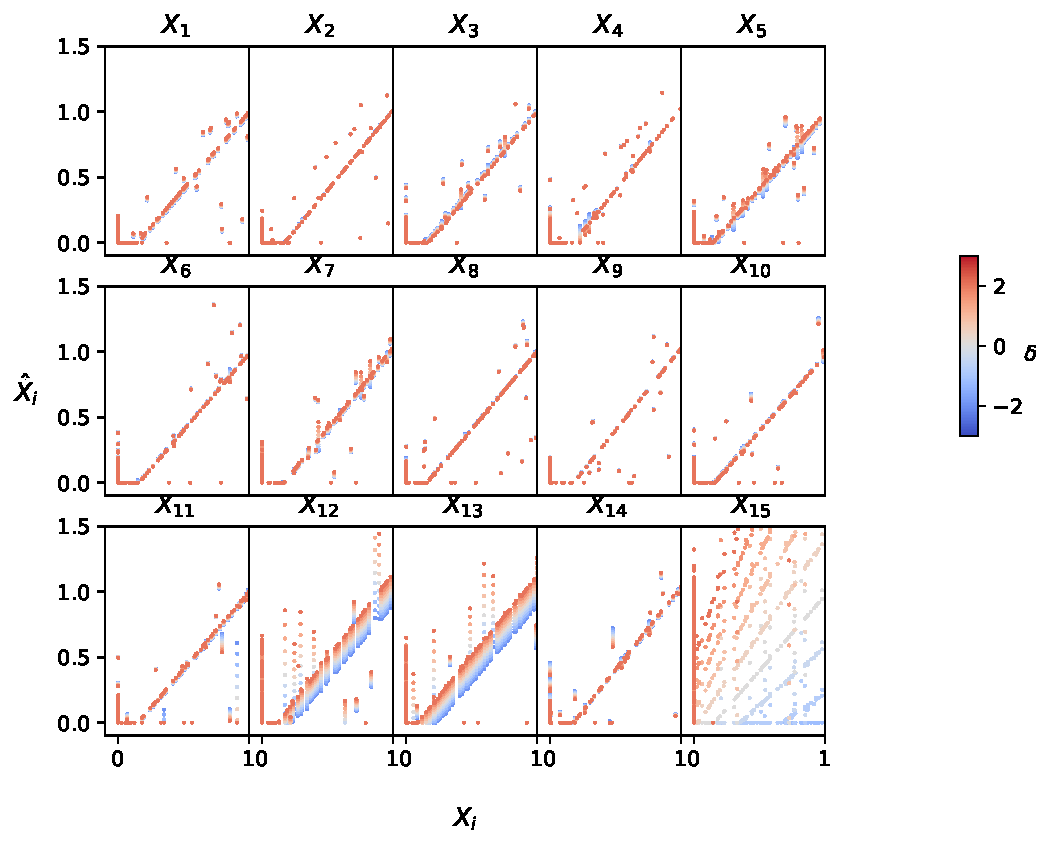
\includegraphics[width=\linewidth]{../figures/s4_tms_intervention_network1.pdf}
                \caption{Subnetwork 1}
            \end{subfigure} &
            \begin{subfigure}{0.3\textwidth}
                \centering
                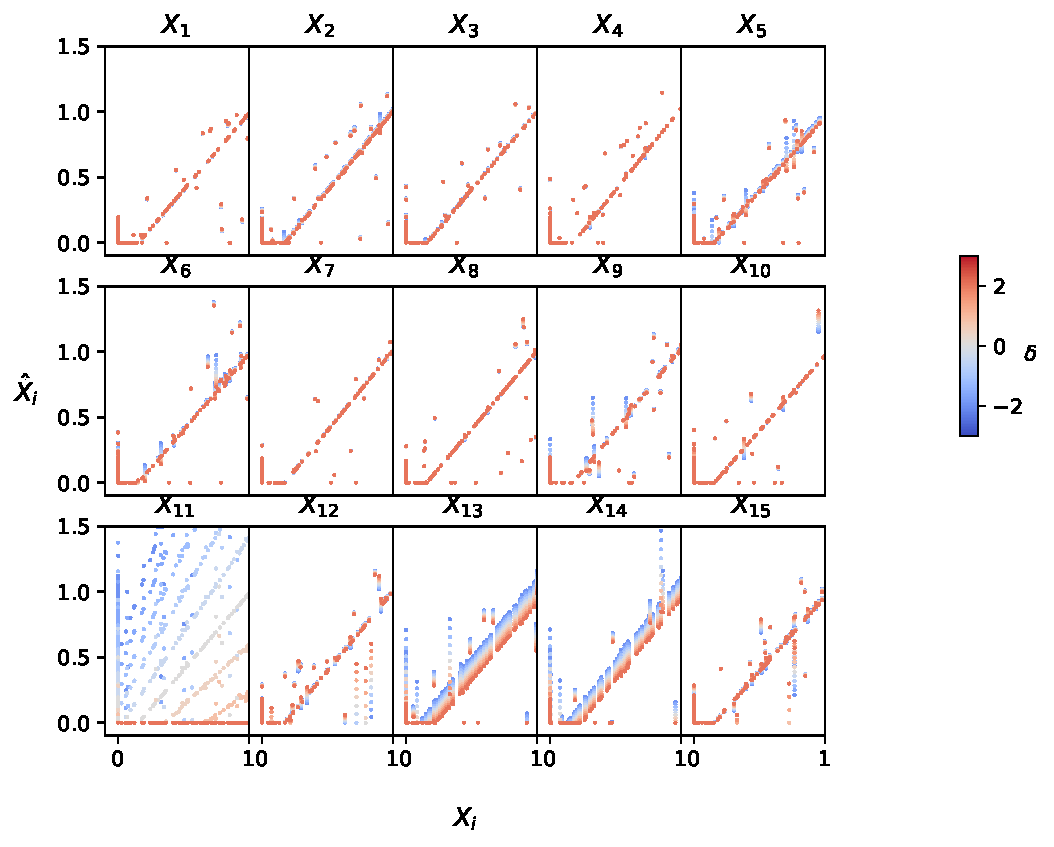
\includegraphics[width=\linewidth]{../figures/s4_tms_intervention_network2.pdf}
                \caption{Subnetwork 2}
            \end{subfigure} \\ % Move to the next row
            \begin{subfigure}{0.3\textwidth}
                \centering
                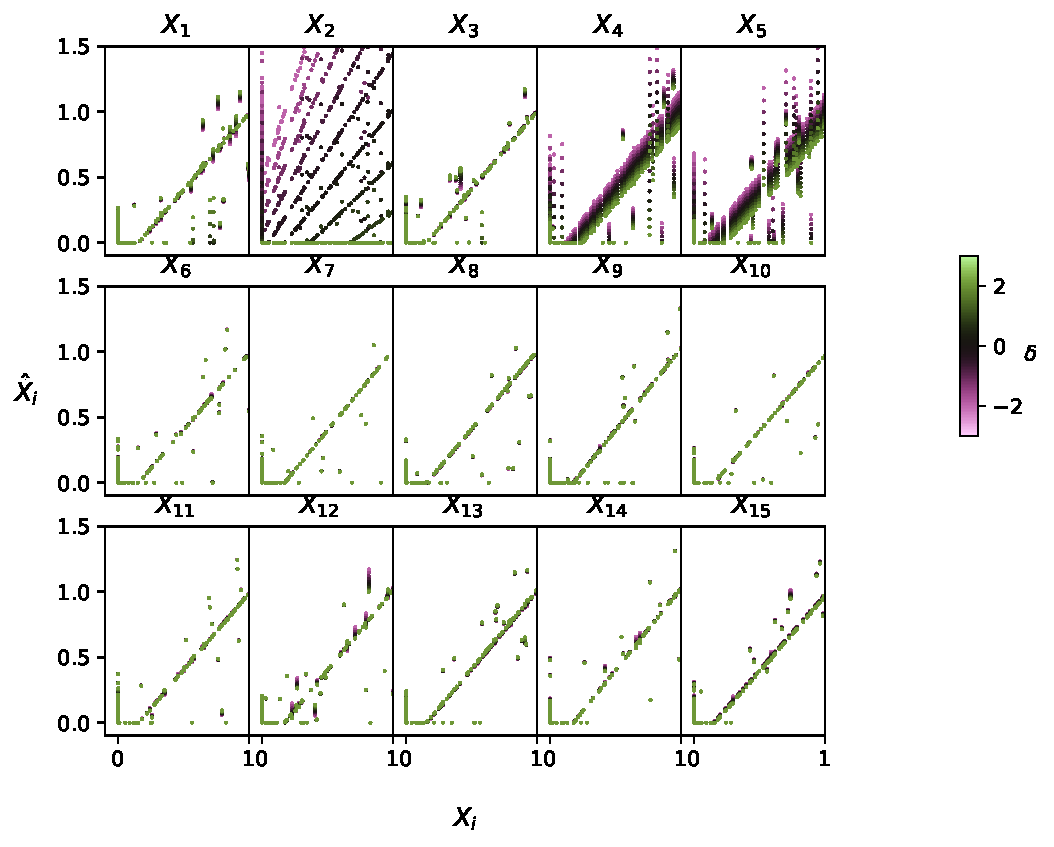
\includegraphics[width=\linewidth]{../figures/s4_tms_intervention_network3.pdf}
                \caption{Subnetwork 3}
            \end{subfigure} & % Move to the next row
            
            \begin{subfigure}{0.3\textwidth}
                \centering
                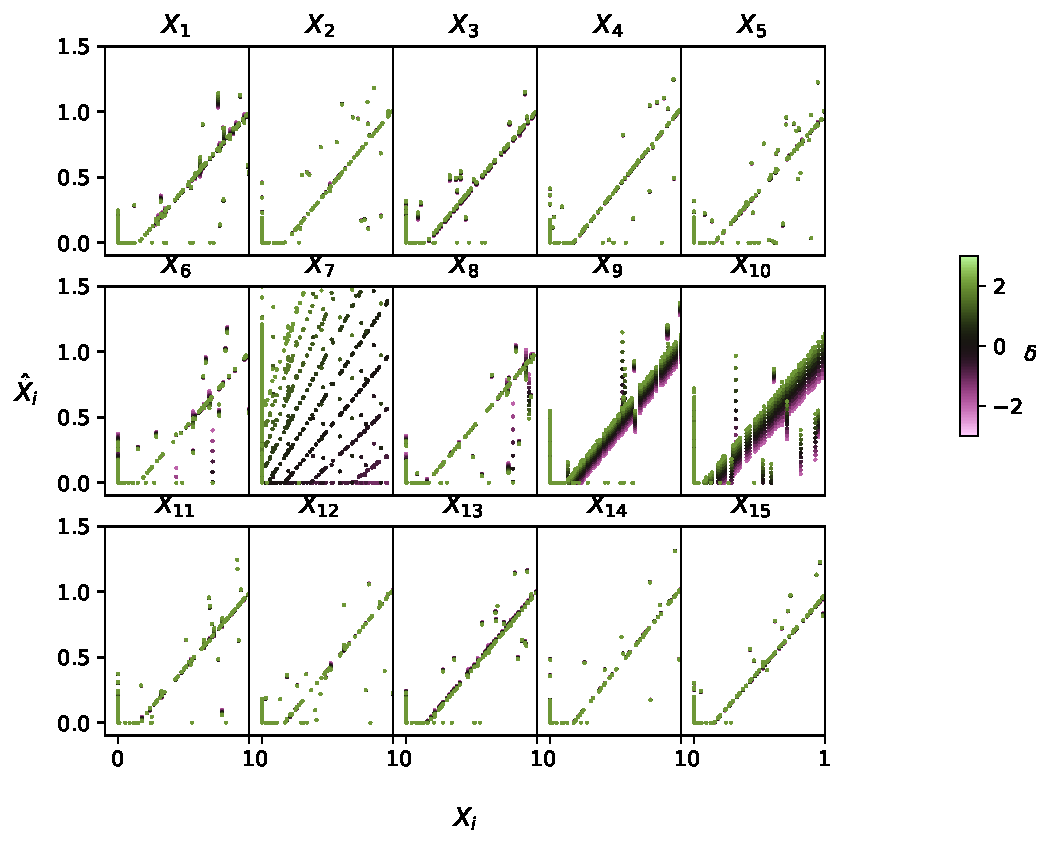
\includegraphics[width=\linewidth]{../figures/s4_tms_intervention_network4.pdf}
                \caption{Subnetwork 4}
            \end{subfigure} \\
            \hspace{\fill} % Spacer to align
            \begin{subfigure}{0.3\textwidth}
                \centering
                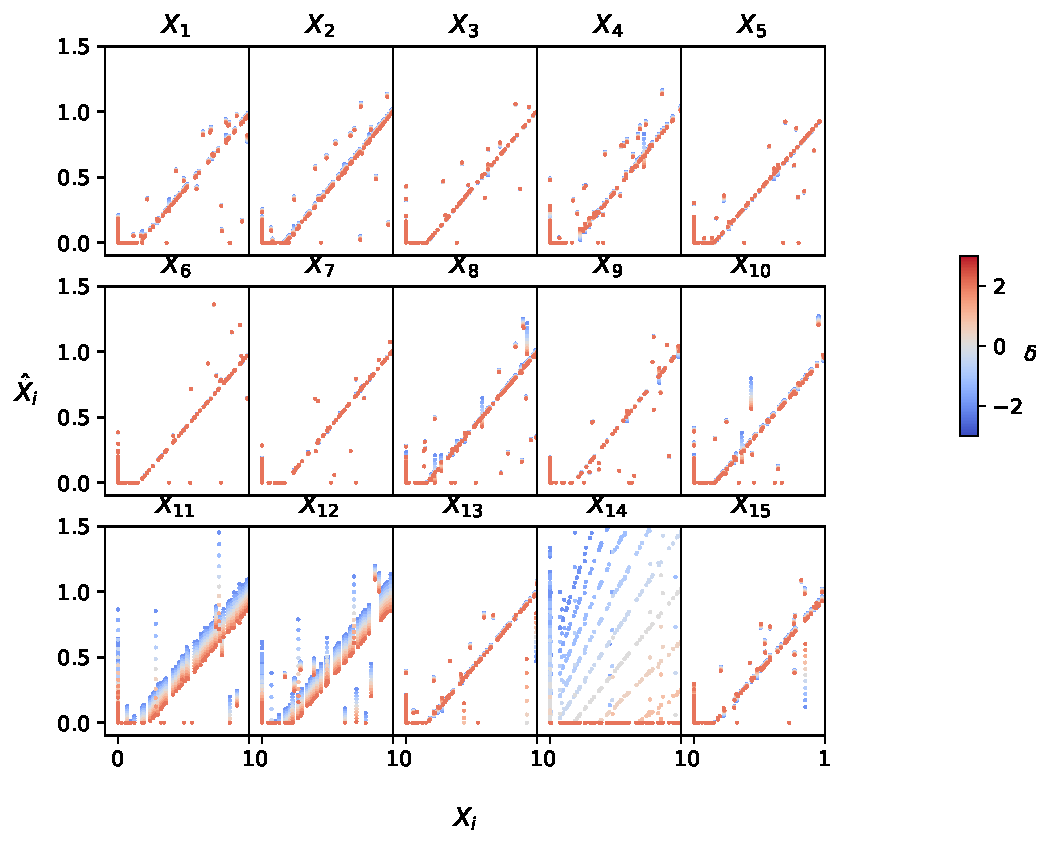
\includegraphics[width=\linewidth]{../figures/s4_tms_intervention_network5.pdf}
                \caption{Subnetwork 5}
            \end{subfigure} &
            \hspace{\fill} % Spacer to align
        \end{tabular}
    \end{minipage}

\end{figure}


%---------------- FIGURE S6: Higher Rank Circuit Superposition ----------------
\begin{figure}[ht]
    \centerline{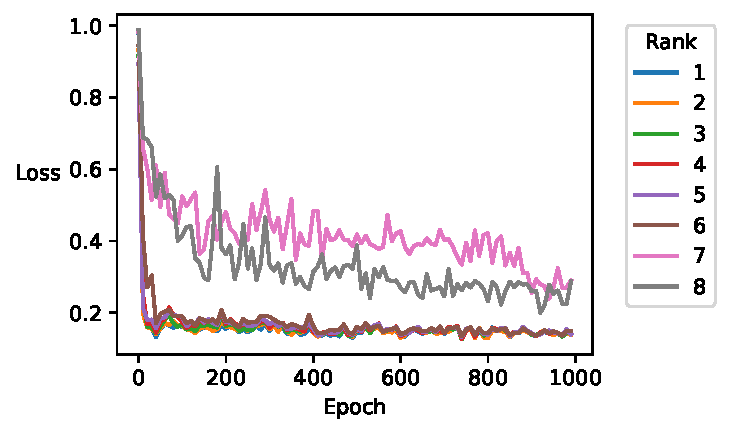
\includegraphics{../figures/s5_high_rank_circuits_loss_vs_rank.pdf}}
    \centering
    \caption{Loss vs Rank}\label{fig:s5_high_rank_circuits_loss_vs_rank}
\end{figure}

  
%--------------- TO DO CIRCUIT DECOMPOSITION RANKFIGURE -------------
\todo{CIRCUIT DECOMPOSITION RANK FIGURE}
\begin{figure}[ht]
    %\centerline{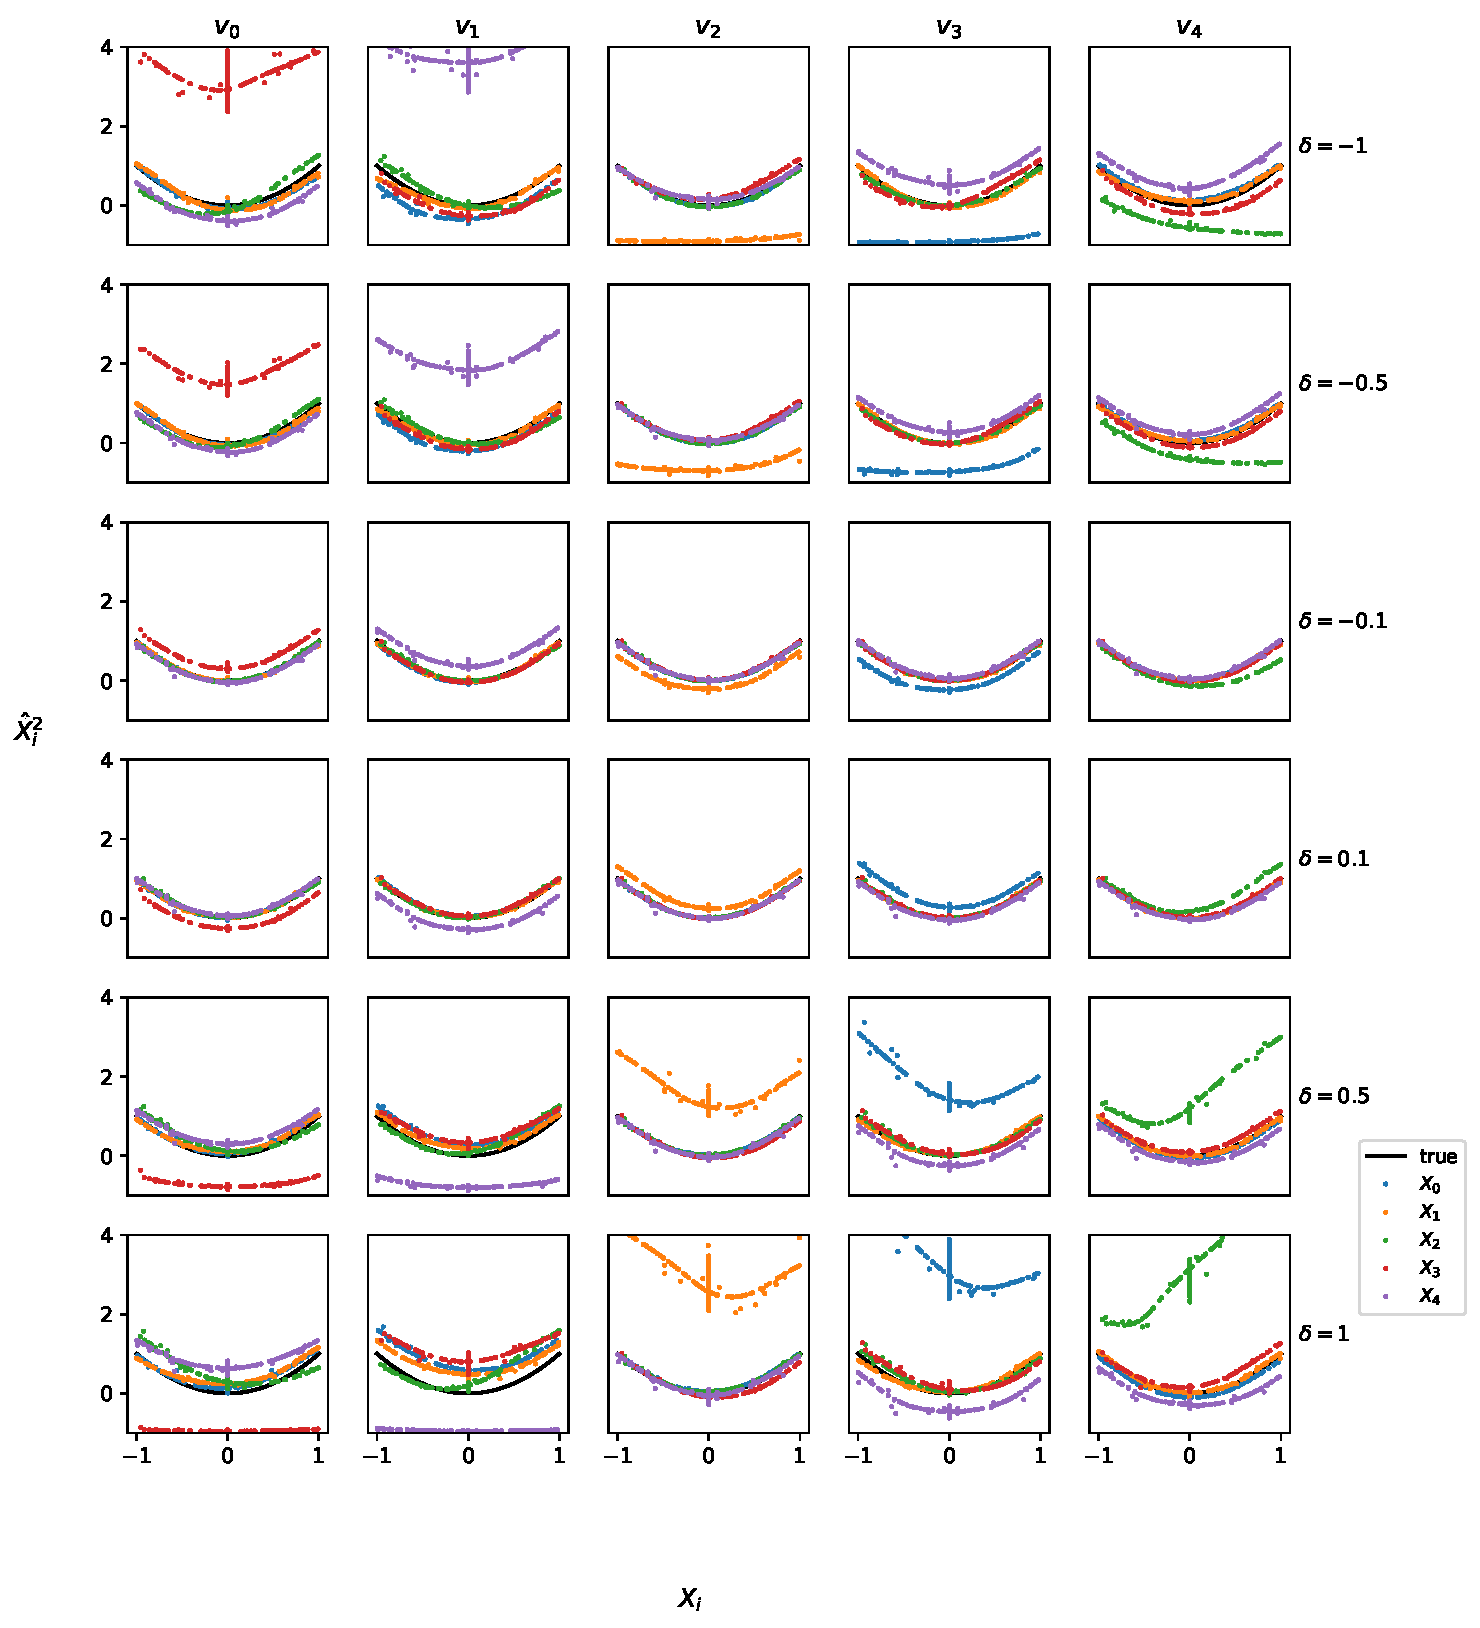
\includegraphics[width=\textwidth]{../figures/s7_squared_intervention_more_deltas.pdf}}
    \centering
    \caption{Decomposition of the high rank circuit model using different rank parameter directions}\label{fig:s8_high_rank_circuit_decomposition_rank}
\end{figure}

%--------------------- FIGURE S7: Squared Model Middle Layer Intervention ---------------------
\begin{figure}[ht]
    \centerline{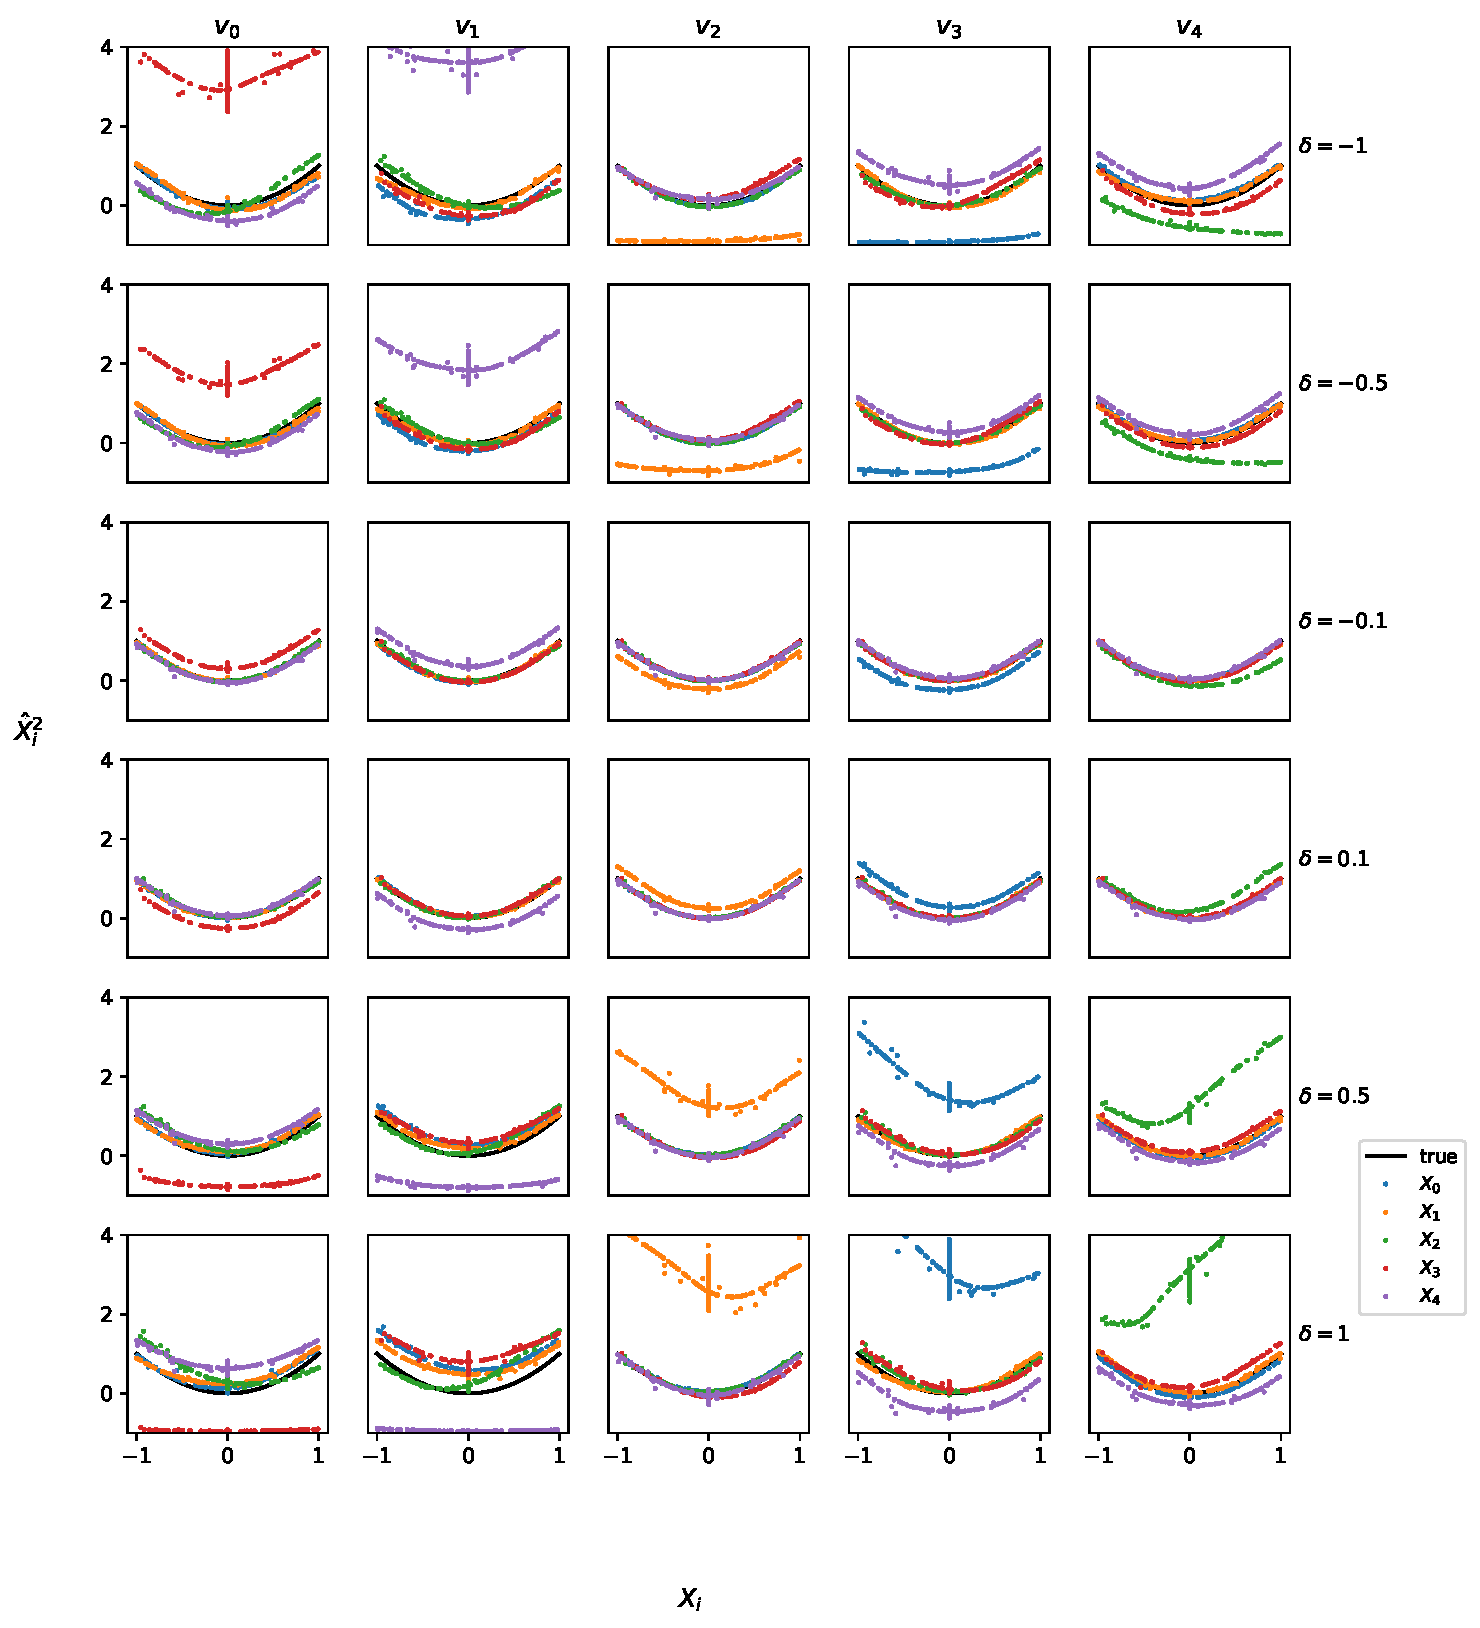
\includegraphics[width=\textwidth]{../figures/s7_squared_intervention_more_deltas.pdf}}
    \centering
    \caption{Effects of intervening on each of the 5 subnetworks of the $X \mapsto X^2$ model.}\label{fig:s7_squared_intervention_more_deltas}
\end{figure}

%--------------------- FIGURE S8: Squared Model Middle Layer Intervention ---------------------
\begin{figure}[ht]
    \centerline{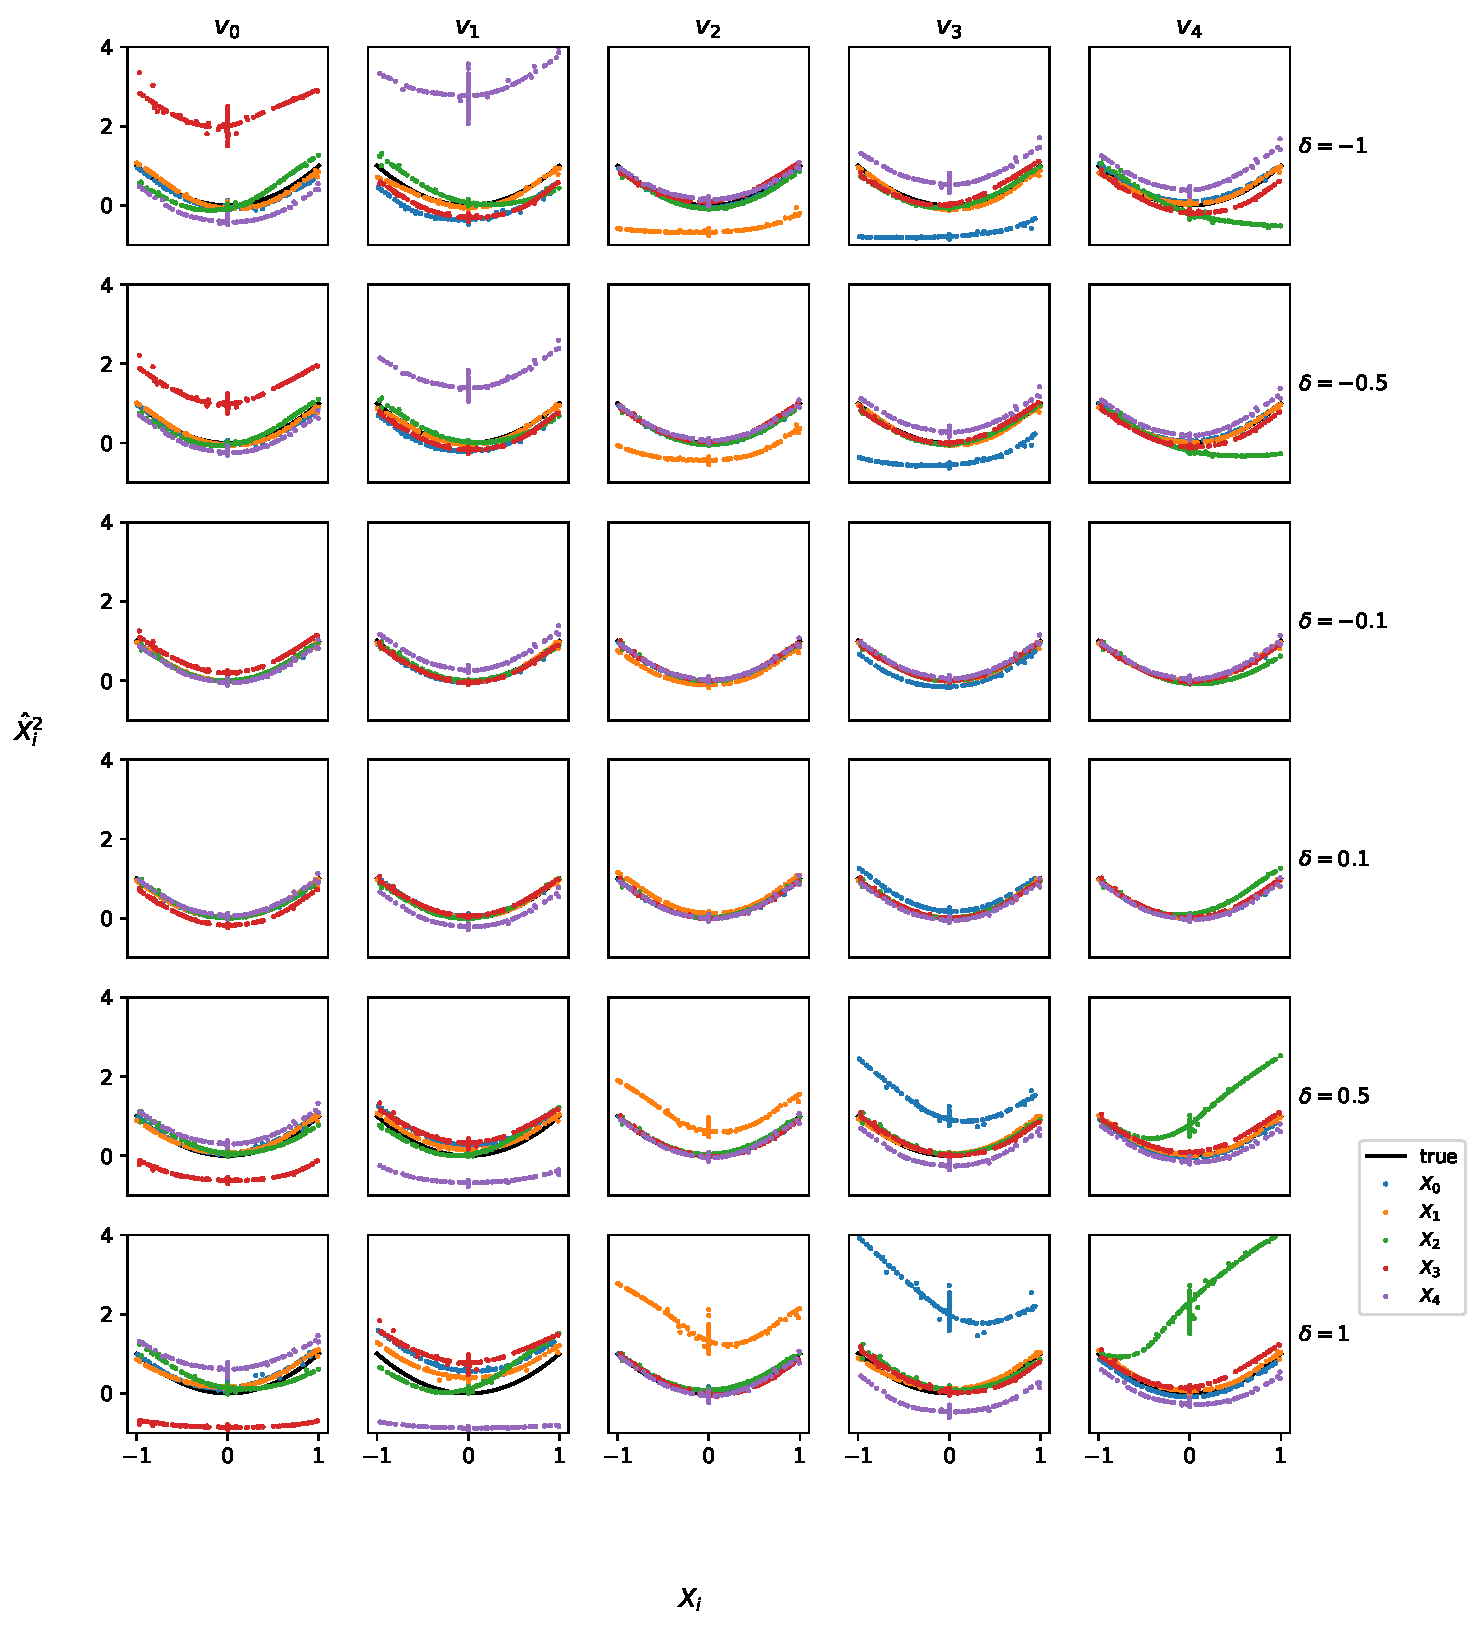
\includegraphics[width=\textwidth]{../figures/s8_squared_intervention_middle_weights.pdf}}
    \centering
    \caption{Intervening on just the weights and biases of the middle hidden layers in the $X \mapsto X^2$ network.}\label{fig:s8_squared_intervention_middle_weights}
\end{figure}


%--------------------- FIGURE S9: Squared Model Multi-Feature Intervention ---------------------
\begin{figure}[ht]
    \centerline{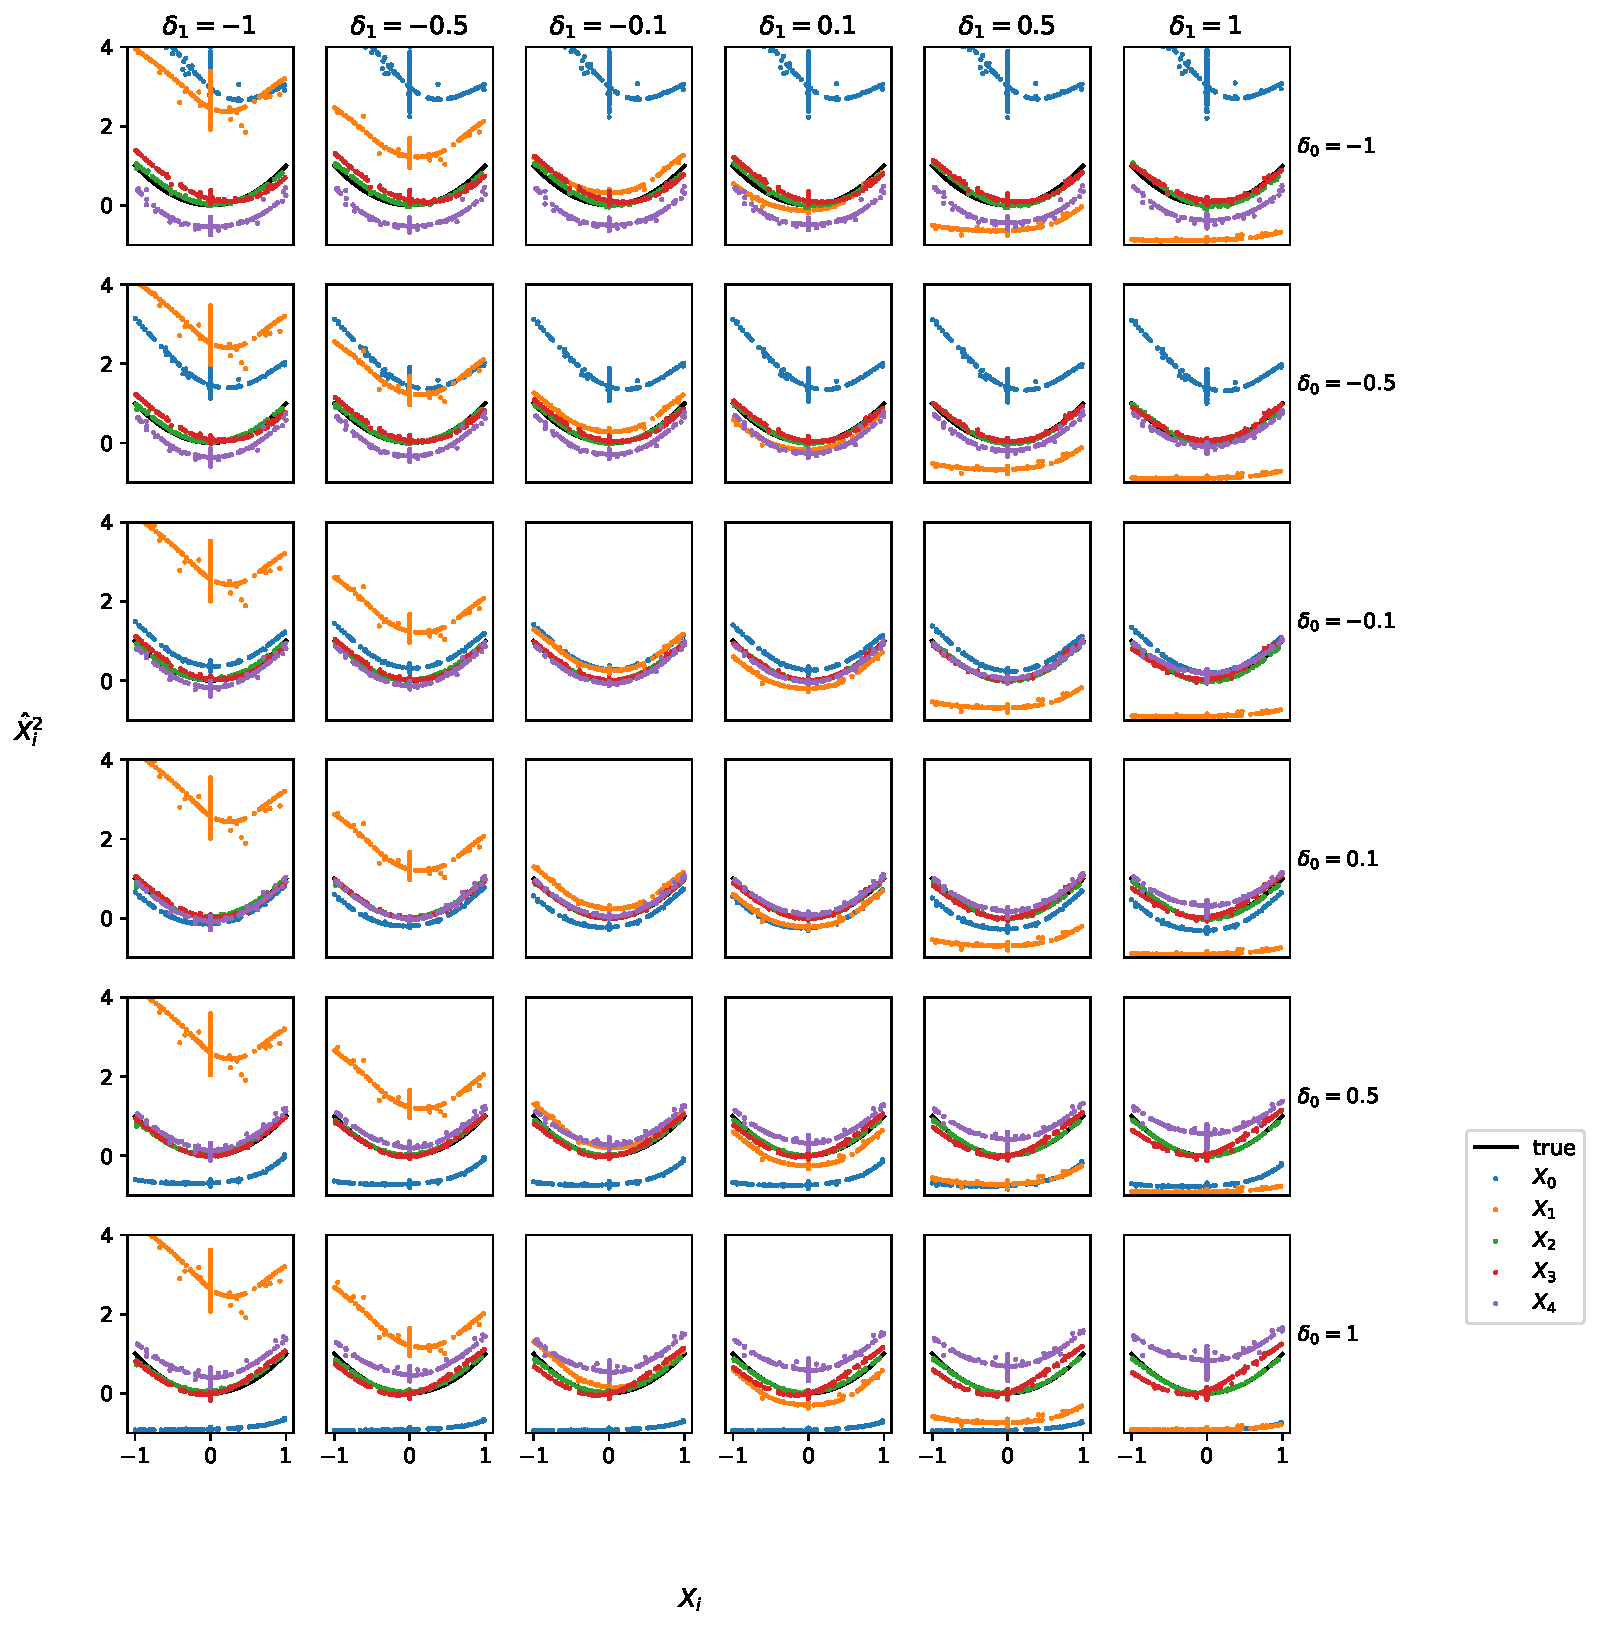
\includegraphics[width=\textwidth]{../figures/s9_squared_intervention_multi_features.pdf}}
    \centering
    \caption{Intervening on multiple subnetworks at once.}\label{fig:s9_squared_intervention_multi_features}
\end{figure}

%--------------------- FIGURE S10: Squared Model Decompositions ---------------------
\begin{figure}[ht]
    %\centerline{\includegraphics[width=\textwidth]{../figures/s10_squared_decompositions_rank.pdf}}
    \centering
    \caption{Decompositions when using different numbers of subnetworks}\label{fig:s10_squared_decompositions_features}
\end{figure}


%--------------------- FIGURE S11: Squared Model Multi-Feature Intervention ---------------------
\begin{figure}[ht]
    %\centerline{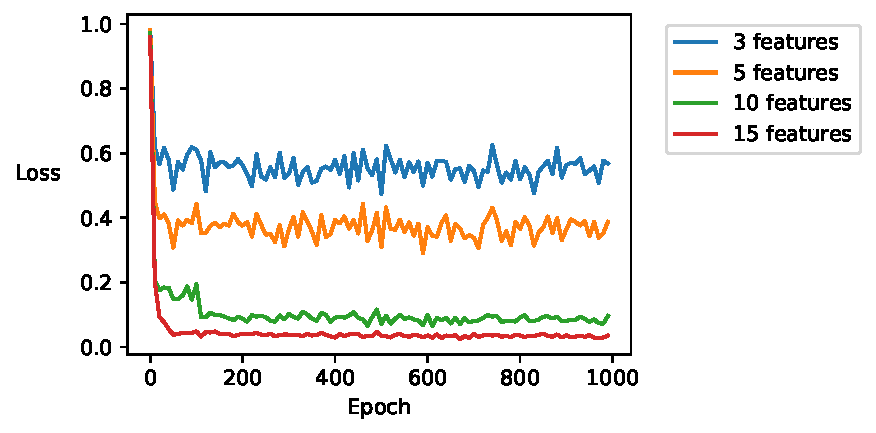
\includegraphics[width=\textwidth]{../figures/s11_squared_features_vs_loss.pdf}}
    \centering
    \caption{Training loss vs number of features for the $X \mapsto X^2$ model, and decompositions for a 3- and 5- subnetwork decomposition.}\label{fig:s11_squared_features_vs_loss}
\end{figure}

\end{document}